\PassOptionsToPackage{loadshadowlibrary}{todonotes}
\RequirePackage[T1]{fontenc}
\RequirePackage[utf8]{inputenc}
%\documentclass[germanthesis,twoside]{vssthesis}
\documentclass[twoside,privacy]{vssthesis}
% options:
% [germanthesis] - Thesis is written in German
% [plainunnumbered] - Don't print numbers on plain pages
% [privacy] - Generate a more privacy aware PDF (exclude birthplace and birthday)
% [twoside] - double sided
% [watermark] - Print current time/date at bottom of each page

\usepackage{array,tabularx,longtable,seqsplit}
\usepackage{pgfplots}
\pgfplotsset{compat=1.18}
\usetikzlibrary{arrows.meta,positioning,shadows}
\usepackage{dataref}
\drefkeys{/pgf/number format/.cd,1000 sep={\,},precision=4}
\newcommand{\dSI}[2]{\drefref{#1}\SI{\drefvalueof{#1}}{#2}}
\newcolumntype{Y}{>{\raggedright\arraybackslash}X}
\newcommand{\filepath}[1]{\path{#1}}
% Generated by prepare_data.py; edit evidence inputs, not this file.
% Source: evidence/current/catalogue.csv SHA-256 ba3951d6219fcade0283d9b41e21d5e8fa91c53be565d6d0dc336ca8fdeee706
\drefset{/catalogue/total}{40}
\drefset{/catalogue/real}{36}
\drefset{/catalogue/control}{1}
\drefset{/catalogue/synthetic}{3}
\drefset{/catalogue/covered}{39}
% Source: evidence/current/tier1-totals.csv SHA-256 b6698505f29ce5614a42576765cebefdd9dc5faaa9d3070691ceaa38e6a05308
\drefset{/tier1/totals/2/n}{2}
\drefset{/tier1/totals/2/combinations}{780}
\drefset{/tier1/totals/2/accept}{667}
\drefset{/tier1/totals/2/reject}{113}
\drefset{/tier1/totals/3/n}{3}
\drefset{/tier1/totals/3/combinations}{9880}
\drefset{/tier1/totals/3/accept}{7807}
\drefset{/tier1/totals/3/reject}{2073}
% Source: evidence/current/tier1-classes.csv SHA-256 4bca7c7ce81d15da826e2bad5fa49e38b794faee2799d13d6e9e18b951f7c70a
\drefset{/tier1/classes/2/n}{2}
\drefset{/tier1/classes/2/reject}{113}
\drefset{/tier1/classes/2/version-skew}{7}
\drefset{/tier1/classes/2/declared-conflict}{1}
\drefset{/tier1/classes/2/file-collision}{0}
\drefset{/tier1/classes/2/identity-collision}{0}
\drefset{/tier1/classes/2/module-relation}{75}
\drefset{/tier1/classes/2/base-drift}{0}
\drefset{/tier1/classes/2/not-composable}{39}
\drefset{/tier1/classes/3/n}{3}
\drefset{/tier1/classes/3/reject}{2073}
\drefset{/tier1/classes/3/version-skew}{245}
\drefset{/tier1/classes/3/declared-conflict}{38}
\drefset{/tier1/classes/3/file-collision}{0}
\drefset{/tier1/classes/3/identity-collision}{0}
\drefset{/tier1/classes/3/module-relation}{1370}
\drefset{/tier1/classes/3/base-drift}{0}
\drefset{/tier1/classes/3/not-composable}{741}
% Source: evidence/current/tier1-measured.csv SHA-256 97de92fcf54cb0088b4cc12f8ecd7cef7468bca4bbd848e1163a2b1c975b2bb3
\drefset{/tier1/measured/2/n}{2}
\drefset{/tier1/measured/2/combinations}{780}
\drefset{/tier1/measured/2/sets-with-benign-overlap}{168}
\drefset{/tier1/measured/2/benign-overlap-instances}{667}
\drefset{/tier1/measured/2/sets-with-suppressed-collision}{1}
\drefset{/tier1/measured/2/suppressed-instances}{4}
\drefset{/tier1/measured/3/n}{3}
\drefset{/tier1/measured/3/combinations}{9880}
\drefset{/tier1/measured/3/sets-with-benign-overlap}{4585}
\drefset{/tier1/measured/3/benign-overlap-instances}{25346}
\drefset{/tier1/measured/3/sets-with-suppressed-collision}{38}
\drefset{/tier1/measured/3/suppressed-instances}{152}
% Source: evidence/current/tier1-crosscheck.csv SHA-256 4311d2f149cb11a871e86e285be4dfe92ccc42550cbc6992b998f89a45a906fd
\drefset{/tier1/crosscheck/3/n}{3}
\drefset{/tier1/crosscheck/3/sets}{9880}
\drefset{/tier1/crosscheck/3/sets-containing-rejecting-pair}{2145}
\drefset{/tier1/crosscheck/3/reject}{2073}
\drefset{/tier1/crosscheck/3/reject-explained}{2073}
\drefset{/tier1/crosscheck/3/reject-unexplained}{0}
\drefset{/tier1/crosscheck/3/accept-despite-rejecting-pair}{72}
% Source: evidence/current/tier1-control.csv SHA-256 34fd65f843aed9e8a7ec9a824d4222fbbc0ac84e89eb49513c6558c2586193da
\drefset{/tier1/control/2/n}{2}
\drefset{/tier1/control/2/predicted}{39}
\drefset{/tier1/control/2/observed}{39}
\drefset{/tier1/control/3/n}{3}
\drefset{/tier1/control/3/predicted}{741}
\drefset{/tier1/control/3/observed}{741}
% Source: evidence/current/tier1-nonmonotone.csv SHA-256 69f233ae068b672506c52786871181262c7ebd19ef7813fa9c3560d6d698eb83
\drefset{/tier1/nonmonotone/3/n}{3}
\drefset{/tier1/nonmonotone/3/containing-sets-admitted}{72}
% Source: evidence/current/tier2-fit.csv SHA-256 07d5f0ec00367d87d5a76b9735bee6bee0c6d8d78fc9ef0190099c4455eb6a05
\drefset{/tier2/current/mount/intercept-ms}{17.4}
\drefset{/tier2/current/mount/slope-ms-per-module}{11.73}
\drefset{/tier2/current/mount/r2}{0.9746}
\drefset{/tier2/current/mount/n}{152}
\drefset{/tier2/current/reconcile/intercept-ms}{74.5}
\drefset{/tier2/current/reconcile/slope-ms-per-module}{18.80}
\drefset{/tier2/current/reconcile/r2}{0.9630}
\drefset{/tier2/current/reconcile/n}{152}
\drefset{/tier2/current/compose/intercept-ms}{92.0}
\drefset{/tier2/current/compose/slope-ms-per-module}{30.53}
\drefset{/tier2/current/compose/r2}{0.9813}
\drefset{/tier2/current/compose/n}{152}
\drefset{/tier2/current/verify/intercept-ms}{96.1}
\drefset{/tier2/current/verify/slope-ms-per-module}{39.08}
\drefset{/tier2/current/verify/r2}{0.9649}
\drefset{/tier2/current/verify/n}{152}
% Source: evidence/previous/tier2-fit.csv SHA-256 24067b86f18cb0c2cdec6bb11737f0e346f79a3a6824b53aaadc9564a86774b2
\drefset{/tier2/previous/mount/intercept-ms}{20.8}
\drefset{/tier2/previous/mount/slope-ms-per-module}{9.46}
\drefset{/tier2/previous/mount/r2}{0.9845}
\drefset{/tier2/previous/mount/n}{152}
\drefset{/tier2/previous/reconcile/intercept-ms}{154.4}
\drefset{/tier2/previous/reconcile/slope-ms-per-module}{21.09}
\drefset{/tier2/previous/reconcile/r2}{0.9577}
\drefset{/tier2/previous/reconcile/n}{152}
\drefset{/tier2/previous/compose/intercept-ms}{175.2}
\drefset{/tier2/previous/compose/slope-ms-per-module}{30.55}
\drefset{/tier2/previous/compose/r2}{0.9747}
\drefset{/tier2/previous/compose/n}{152}
\drefset{/tier2/previous/verify/intercept-ms}{161.3}
\drefset{/tier2/previous/verify/slope-ms-per-module}{41.80}
\drefset{/tier2/previous/verify/r2}{0.9605}
\drefset{/tier2/previous/verify/n}{152}
% Source: evidence/current/tier2-by-n.csv SHA-256 fb8f80a68c82ed0d66a33c1e8ae6cb89c42f8dc420ee54f151949a132cc95066
\drefset{/timing/2/n}{2}
\drefset{/timing/2/samples}{30}
\drefset{/timing/2/mount-ms-mean}{46}
\drefset{/timing/2/reconcile-ms-mean}{114}
\drefset{/timing/2/total-ms-mean}{160}
\drefset{/timing/2/verify-ms-mean}{175}
\drefset{/timing/2/packages-min}{117}
\drefset{/timing/2/packages-max}{178}
\drefset{/timing/2/alt-groups-min}{5}
\drefset{/timing/2/alt-groups-max}{38}
\drefset{/timing/2/debconf-records-min}{90}
\drefset{/timing/2/debconf-records-max}{114}
\drefset{/timing/3/n}{3}
\drefset{/timing/3/samples}{30}
\drefset{/timing/3/mount-ms-mean}{56}
\drefset{/timing/3/reconcile-ms-mean}{118}
\drefset{/timing/3/total-ms-mean}{173}
\drefset{/timing/3/verify-ms-mean}{205}
\drefset{/timing/3/packages-min}{126}
\drefset{/timing/3/packages-max}{187}
\drefset{/timing/3/alt-groups-min}{5}
\drefset{/timing/3/alt-groups-max}{17}
\drefset{/timing/3/debconf-records-min}{90}
\drefset{/timing/3/debconf-records-max}{156}
\drefset{/timing/5/n}{5}
\drefset{/timing/5/samples}{20}
\drefset{/timing/5/mount-ms-mean}{75}
\drefset{/timing/5/reconcile-ms-mean}{174}
\drefset{/timing/5/total-ms-mean}{249}
\drefset{/timing/5/verify-ms-mean}{305}
\drefset{/timing/5/packages-min}{131}
\drefset{/timing/5/packages-max}{216}
\drefset{/timing/5/alt-groups-min}{5}
\drefset{/timing/5/alt-groups-max}{52}
\drefset{/timing/5/debconf-records-min}{90}
\drefset{/timing/5/debconf-records-max}{156}
\drefset{/timing/10/n}{10}
\drefset{/timing/10/samples}{10}
\drefset{/timing/10/mount-ms-mean}{128}
\drefset{/timing/10/reconcile-ms-mean}{256}
\drefset{/timing/10/total-ms-mean}{384}
\drefset{/timing/10/verify-ms-mean}{460}
\drefset{/timing/10/packages-min}{174}
\drefset{/timing/10/packages-max}{273}
\drefset{/timing/10/alt-groups-min}{7}
\drefset{/timing/10/alt-groups-max}{49}
\drefset{/timing/10/debconf-records-min}{90}
\drefset{/timing/10/debconf-records-max}{156}
\drefset{/timing/15/n}{15}
\drefset{/timing/15/samples}{10}
\drefset{/timing/15/mount-ms-mean}{188}
\drefset{/timing/15/reconcile-ms-mean}{380}
\drefset{/timing/15/total-ms-mean}{567}
\drefset{/timing/15/verify-ms-mean}{680}
\drefset{/timing/15/packages-min}{224}
\drefset{/timing/15/packages-max}{305}
\drefset{/timing/15/alt-groups-min}{12}
\drefset{/timing/15/alt-groups-max}{54}
\drefset{/timing/15/debconf-records-min}{100}
\drefset{/timing/15/debconf-records-max}{164}
\drefset{/timing/20/n}{20}
\drefset{/timing/20/samples}{10}
\drefset{/timing/20/mount-ms-mean}{237}
\drefset{/timing/20/reconcile-ms-mean}{468}
\drefset{/timing/20/total-ms-mean}{706}
\drefset{/timing/20/verify-ms-mean}{903}
\drefset{/timing/20/packages-min}{230}
\drefset{/timing/20/packages-max}{351}
\drefset{/timing/20/alt-groups-min}{14}
\drefset{/timing/20/alt-groups-max}{68}
\drefset{/timing/20/debconf-records-min}{112}
\drefset{/timing/20/debconf-records-max}{172}
\drefset{/timing/25/n}{25}
\drefset{/timing/25/samples}{10}
\drefset{/timing/25/mount-ms-mean}{298}
\drefset{/timing/25/reconcile-ms-mean}{573}
\drefset{/timing/25/total-ms-mean}{872}
\drefset{/timing/25/verify-ms-mean}{1103}
\drefset{/timing/25/packages-min}{307}
\drefset{/timing/25/packages-max}{371}
\drefset{/timing/25/alt-groups-min}{26}
\drefset{/timing/25/alt-groups-max}{67}
\drefset{/timing/25/debconf-records-min}{120}
\drefset{/timing/25/debconf-records-max}{166}
\drefset{/timing/27/n}{27}
\drefset{/timing/27/samples}{10}
\drefset{/timing/27/mount-ms-mean}{321}
\drefset{/timing/27/reconcile-ms-mean}{597}
\drefset{/timing/27/total-ms-mean}{918}
\drefset{/timing/27/verify-ms-mean}{1180}
\drefset{/timing/27/packages-min}{325}
\drefset{/timing/27/packages-max}{383}
\drefset{/timing/27/alt-groups-min}{29}
\drefset{/timing/27/alt-groups-max}{67}
\drefset{/timing/27/debconf-records-min}{114}
\drefset{/timing/27/debconf-records-max}{174}
\drefset{/timing/30/n}{30}
\drefset{/timing/30/samples}{10}
\drefset{/timing/30/mount-ms-mean}{359}
\drefset{/timing/30/reconcile-ms-mean}{617}
\drefset{/timing/30/total-ms-mean}{976}
\drefset{/timing/30/verify-ms-mean}{1238}
\drefset{/timing/30/packages-min}{339}
\drefset{/timing/30/packages-max}{381}
\drefset{/timing/30/alt-groups-min}{25}
\drefset{/timing/30/alt-groups-max}{67}
\drefset{/timing/30/debconf-records-min}{112}
\drefset{/timing/30/debconf-records-max}{174}
\drefset{/timing/33/n}{33}
\drefset{/timing/33/samples}{6}
\drefset{/timing/33/mount-ms-mean}{437}
\drefset{/timing/33/reconcile-ms-mean}{674}
\drefset{/timing/33/total-ms-mean}{1111}
\drefset{/timing/33/verify-ms-mean}{1350}
\drefset{/timing/33/packages-min}{367}
\drefset{/timing/33/packages-max}{395}
\drefset{/timing/33/alt-groups-min}{34}
\drefset{/timing/33/alt-groups-max}{68}
\drefset{/timing/33/debconf-records-min}{118}
\drefset{/timing/33/debconf-records-max}{168}
\drefset{/timing/35/n}{35}
\drefset{/timing/35/samples}{4}
\drefset{/timing/35/mount-ms-mean}{455}
\drefset{/timing/35/reconcile-ms-mean}{703}
\drefset{/timing/35/total-ms-mean}{1158}
\drefset{/timing/35/verify-ms-mean}{1454}
\drefset{/timing/35/packages-min}{388}
\drefset{/timing/35/packages-max}{408}
\drefset{/timing/35/alt-groups-min}{35}
\drefset{/timing/35/alt-groups-max}{68}
\drefset{/timing/35/debconf-records-min}{172}
\drefset{/timing/35/debconf-records-max}{174}
\drefset{/timing/38/n}{38}
\drefset{/timing/38/samples}{2}
\drefset{/timing/38/alt-groups}{68}
\drefset{/timing/38/mount-ms-mean}{504}
\drefset{/timing/38/reconcile-ms-mean}{764}
\drefset{/timing/38/total-ms-mean}{1268}
\drefset{/timing/38/verify-ms-mean}{1582}
\drefset{/timing/38/packages-min}{406}
\drefset{/timing/38/packages-max}{413}
\drefset{/timing/38/alt-groups-min}{68}
\drefset{/timing/38/alt-groups-max}{68}
\drefset{/timing/38/debconf-records-min}{168}
\drefset{/timing/38/debconf-records-max}{174}
% Source: evidence/current/tier2-checks.csv SHA-256 fde1c2697cd986acc202c77306a5ebebcb72d4d397803728b6d69cdaff8159d1
\drefset{/checks/V1/passing}{152}
\drefset{/checks/V1/total}{152}
\drefset{/checks/V2/passing}{152}
\drefset{/checks/V2/total}{152}
\drefset{/checks/V3/passing}{152}
\drefset{/checks/V3/total}{152}
\drefset{/checks/V4/passing}{152}
\drefset{/checks/V4/total}{152}
\drefset{/checks/V5/passing}{152}
\drefset{/checks/V5/total}{152}
\drefset{/checks/V6/passing}{152}
\drefset{/checks/V6/total}{152}
\drefset{/checks/V7/passing}{152}
\drefset{/checks/V7/total}{152}
\drefset{/checks/V8/passing}{152}
\drefset{/checks/V8/total}{152}
% Source: evidence/current/storage-cohorts.csv SHA-256 b5b065efe366840b063c25ad880df31e6a8360d7f883e26c055b31dcf673d81e
\drefset{/storage/small/n}{31}
\drefset{/storage/small/stored-mb}{282.6}
\drefset{/storage/small/monolithic-mb}{1534.2}
\drefset{/storage/small/ratio}{5.43}
\drefset{/storage/small/mean-delta-mb}{7.8}
\drefset{/storage/large/n}{9}
\drefset{/storage/large/stored-mb}{1704.5}
\drefset{/storage/large/monolithic-mb}{2038.3}
\drefset{/storage/large/ratio}{1.20}
\drefset{/storage/large/mean-delta-mb}{184.8}
\drefset{/storage/all/n}{40}
\drefset{/storage/all/stored-mb}{1945.4}
\drefset{/storage/all/monolithic-mb}{3572.4}
\drefset{/storage/all/ratio}{1.84}
\drefset{/storage/all/mean-delta-mb}{47.6}
% Source: evidence/current/storage-per-module.csv SHA-256 eca500b382a74f1ea7c54d440127f4ae6506508e6ecd5a1d822a9051e426d595
\drefset{/module/cuda-runtime/delta-mb}{680.2}
\drefset{/module/cuda-runtime/monolithic-mb}{721.9}
\drefset{/module/cuda-runtime/saving-pct}{5.8}
\drefset{/module/nvidia-driver-535/delta-mb}{231.6}
\drefset{/module/nvidia-driver-535/monolithic-mb}{273.3}
\drefset{/module/nvidia-driver-535/saving-pct}{15.3}
\drefset{/module/rust/delta-mb}{175.5}
\drefset{/module/rust/monolithic-mb}{217.2}
\drefset{/module/rust/saving-pct}{19.2}
\drefset{/module/java/delta-mb}{141.6}
\drefset{/module/java/monolithic-mb}{183.3}
\drefset{/module/java/saving-pct}{22.8}
\drefset{/module/llvm/delta-mb}{128.2}
\drefset{/module/llvm/monolithic-mb}{169.9}
\drefset{/module/llvm/saving-pct}{24.6}
\drefset{/module/gcc/delta-mb}{84.0}
\drefset{/module/gcc/monolithic-mb}{125.7}
\drefset{/module/gcc/saving-pct}{33.2}
\drefset{/module/docker/delta-mb}{83.1}
\drefset{/module/docker/monolithic-mb}{124.8}
\drefset{/module/docker/saving-pct}{33.4}
\drefset{/module/postgres/delta-mb}{82.1}
\drefset{/module/postgres/monolithic-mb}{123.9}
\drefset{/module/postgres/saving-pct}{33.7}
\drefset{/module/mysql/delta-mb}{56.6}
\drefset{/module/mysql/monolithic-mb}{98.3}
\drefset{/module/mysql/saving-pct}{42.4}
\drefset{/module/emacs/delta-mb}{37.0}
\drefset{/module/emacs/monolithic-mb}{78.7}
\drefset{/module/emacs/saving-pct}{53.0}
\drefset{/module/apache/delta-mb}{28.1}
\drefset{/module/apache/monolithic-mb}{69.8}
\drefset{/module/apache/saving-pct}{59.7}
\drefset{/module/pytools/delta-mb}{25.8}
\drefset{/module/pytools/monolithic-mb}{67.6}
\drefset{/module/pytools/saving-pct}{61.7}
\drefset{/module/webserver/delta-mb}{21.0}
\drefset{/module/webserver/monolithic-mb}{62.8}
\drefset{/module/webserver/saving-pct}{66.5}
\drefset{/module/vim/delta-mb}{18.1}
\drefset{/module/vim/monolithic-mb}{59.8}
\drefset{/module/vim/saving-pct}{69.7}
\drefset{/module/git/delta-mb}{17.1}
\drefset{/module/git/monolithic-mb}{58.9}
\drefset{/module/git/saving-pct}{70.9}
\drefset{/module/dnsutils/delta-mb}{16.0}
\drefset{/module/dnsutils/monolithic-mb}{57.7}
\drefset{/module/dnsutils/saving-pct}{72.3}
\drefset{/module/pipdemo/delta-mb}{15.5}
\drefset{/module/pipdemo/monolithic-mb}{57.2}
\drefset{/module/pipdemo/saving-pct}{72.9}
\drefset{/module/pgclient/delta-mb}{12.1}
\drefset{/module/pgclient/monolithic-mb}{53.8}
\drefset{/module/pgclient/saving-pct}{77.6}
\drefset{/module/jq/delta-mb}{10.4}
\drefset{/module/jq/monolithic-mb}{52.2}
\drefset{/module/jq/saving-pct}{80.0}
\drefset{/module/memcached/delta-mb}{10.3}
\drefset{/module/memcached/monolithic-mb}{52.0}
\drefset{/module/memcached/saving-pct}{80.3}
\drefset{/module/pyyaml/delta-mb}{10.1}
\drefset{/module/pyyaml/monolithic-mb}{51.9}
\drefset{/module/pyyaml/saving-pct}{80.4}
\drefset{/module/gawk/delta-mb}{3.1}
\drefset{/module/gawk/monolithic-mb}{44.8}
\drefset{/module/gawk/saving-pct}{93.1}
\drefset{/module/mta-msmtp/delta-mb}{2.6}
\drefset{/module/mta-msmtp/monolithic-mb}{44.3}
\drefset{/module/mta-msmtp/saving-pct}{94.2}
\drefset{/module/sqlite/delta-mb}{1.9}
\drefset{/module/sqlite/monolithic-mb}{43.6}
\drefset{/module/sqlite/saving-pct}{95.6}
\drefset{/module/redis/delta-mb}{1.7}
\drefset{/module/redis/monolithic-mb}{43.4}
\drefset{/module/redis/saving-pct}{96.2}
\drefset{/module/control-oldsnap/delta-mb}{1.6}
\drefset{/module/control-oldsnap/monolithic-mb}{43.4}
\drefset{/module/control-oldsnap/saving-pct}{96.2}
\drefset{/module/curl/delta-mb}{1.6}
\drefset{/module/curl/monolithic-mb}{43.4}
\drefset{/module/curl/saving-pct}{96.2}
\drefset{/module/tcpdump/delta-mb}{1.1}
\drefset{/module/tcpdump/monolithic-mb}{42.8}
\drefset{/module/tcpdump/saving-pct}{97.5}
\drefset{/module/zstd/delta-mb}{0.9}
\drefset{/module/zstd/monolithic-mb}{42.6}
\drefset{/module/zstd/saving-pct}{98.0}
\drefset{/module/tmux/delta-mb}{0.7}
\drefset{/module/tmux/monolithic-mb}{42.5}
\drefset{/module/tmux/saving-pct}{98.2}
\drefset{/module/rsync/delta-mb}{0.7}
\drefset{/module/rsync/monolithic-mb}{42.4}
\drefset{/module/rsync/saving-pct}{98.4}
\drefset{/module/socat/delta-mb}{0.6}
\drefset{/module/socat/monolithic-mb}{42.3}
\drefset{/module/socat/saving-pct}{98.5}
\drefset{/module/wget/delta-mb}{0.6}
\drefset{/module/wget/monolithic-mb}{42.3}
\drefset{/module/wget/saving-pct}{98.6}
\drefset{/module/mta-nullmailer/delta-mb}{0.5}
\drefset{/module/mta-nullmailer/monolithic-mb}{42.2}
\drefset{/module/mta-nullmailer/saving-pct}{98.9}
\drefset{/module/htop/delta-mb}{0.4}
\drefset{/module/htop/monolithic-mb}{42.1}
\drefset{/module/htop/saving-pct}{99.1}
\drefset{/module/nc-openbsd/delta-mb}{0.3}
\drefset{/module/nc-openbsd/monolithic-mb}{42.0}
\drefset{/module/nc-openbsd/saving-pct}{99.3}
\drefset{/module/original-awk/delta-mb}{0.3}
\drefset{/module/original-awk/monolithic-mb}{42.0}
\drefset{/module/original-awk/saving-pct}{99.3}
\drefset{/module/nc-traditional/delta-mb}{0.3}
\drefset{/module/nc-traditional/monolithic-mb}{42.0}
\drefset{/module/nc-traditional/saving-pct}{99.4}
\drefset{/module/fake-nvidia-driver/delta-mb}{0.2}
\drefset{/module/fake-nvidia-driver/monolithic-mb}{41.9}
\drefset{/module/fake-nvidia-driver/saving-pct}{99.5}
\drefset{/module/fake-cuda/delta-mb}{0.2}
\drefset{/module/fake-cuda/monolithic-mb}{41.9}
\drefset{/module/fake-cuda/saving-pct}{99.5}
% Source: evidence/current/storage-model-check.csv SHA-256 d1a770f0038d7cfb65d286c1afa8c7a0071686428b3da944998b7095cc39cdae
\drefset{/calibration/curl/measured-mb}{43.0}
\drefset{/calibration/curl/modelled-mb}{43.4}
\drefset{/calibration/curl/model-error-pct}{+0.91}
\drefset{/calibration/emacs/measured-mb}{78.3}
\drefset{/calibration/emacs/modelled-mb}{78.7}
\drefset{/calibration/emacs/model-error-pct}{+0.51}
\drefset{/calibration/jq/measured-mb}{51.5}
\drefset{/calibration/jq/modelled-mb}{52.2}
\drefset{/calibration/jq/model-error-pct}{+1.34}
\drefset{/calibration/nc-traditional/measured-mb}{41.6}
\drefset{/calibration/nc-traditional/modelled-mb}{42.0}
\drefset{/calibration/nc-traditional/model-error-pct}{+0.95}
\drefset{/calibration/pytools/measured-mb}{67.4}
\drefset{/calibration/pytools/modelled-mb}{67.6}
\drefset{/calibration/pytools/model-error-pct}{+0.25}
\drefset{/calibration/webserver/measured-mb}{62.3}
\drefset{/calibration/webserver/modelled-mb}{62.8}
\drefset{/calibration/webserver/model-error-pct}{+0.82}
% Source: evidence/current/storage-sensitivity.csv SHA-256 a8a62be93a979cc0a231f5ef8fb0f2f589883810e53fb44f6710a4397272e64b
\drefset{/sensitivity/0/n}{40}
\drefset{/sensitivity/0/stored-mb}{1945.4}
\drefset{/sensitivity/0/monolithic-mb}{3572.4}
\drefset{/sensitivity/0/ratio}{1.84}
\drefset{/sensitivity/0/mean-delta-mb}{47.6}
\drefset{/sensitivity/1/n}{31}
\drefset{/sensitivity/1/stored-mb}{282.6}
\drefset{/sensitivity/1/monolithic-mb}{1534.2}
\drefset{/sensitivity/1/ratio}{5.43}
\drefset{/sensitivity/1/mean-delta-mb}{7.8}
\drefset{/sensitivity/2/n}{36}
\drefset{/sensitivity/2/stored-mb}{1927.8}
\drefset{/sensitivity/2/monolithic-mb}{3388.0}
\drefset{/sensitivity/2/ratio}{1.76}
\drefset{/sensitivity/2/mean-delta-mb}{52.4}
\drefset{/sensitivity/3/n}{39}
\drefset{/sensitivity/3/stored-mb}{1265.2}
\drefset{/sensitivity/3/monolithic-mb}{2850.5}
\drefset{/sensitivity/3/ratio}{2.25}
\drefset{/sensitivity/3/mean-delta-mb}{31.4}
\drefset{/sensitivity/4/n}{39}
\drefset{/sensitivity/4/stored-mb}{1713.9}
\drefset{/sensitivity/4/monolithic-mb}{3299.1}
\drefset{/sensitivity/4/ratio}{1.92}
\drefset{/sensitivity/4/mean-delta-mb}{42.9}
\drefset{/sensitivity/5/n}{39}
\drefset{/sensitivity/5/stored-mb}{1770.0}
\drefset{/sensitivity/5/monolithic-mb}{3355.2}
\drefset{/sensitivity/5/ratio}{1.90}
\drefset{/sensitivity/5/mean-delta-mb}{44.3}
\drefset{/storage/base-mb}{41.7}
% Source: evidence/current/tier3.csv SHA-256 e5edb5f45b5f878e31111003b71b8a6a5b01047be88268650c31922d4fbc3ead
\drefset{/boot/bundles}{20}
\drefset{/boot/current}{2}
\drefset{/boot/pass}{6}
\drefset{/boot/fail}{5}
\drefset{/boot/broken}{2}
\drefset{/boot/aborted}{4}
\drefset{/boot/no-result}{3}
\drefset{/boot/run/0/n}{2}
\drefset{/boot/run/0/exit-code}{0}
\drefset{/boot/run/0/duration-s}{330}
\drefset{/boot/run/1/n}{2}
\drefset{/boot/run/1/exit-code}{2}
\drefset{/boot/run/1/duration-s}{170}
\drefset{/boot/run/2/n}{2}
\drefset{/boot/run/2/exit-code}{2}
\drefset{/boot/run/2/duration-s}{324}
\drefset{/boot/run/3/n}{2}
\drefset{/boot/run/3/exit-code}{2}
\drefset{/boot/run/3/duration-s}{331}
\drefset{/boot/run/4/n}{2}
\drefset{/boot/run/4/exit-code}{0}
\drefset{/boot/run/4/duration-s}{316}
\drefset{/boot/run/5/n}{36}
\drefset{/boot/run/5/exit-code}{1}
\drefset{/boot/run/5/duration-s}{3}
\drefset{/boot/run/6/n}{36}
\drefset{/boot/run/6/exit-code}{0}
\drefset{/boot/run/6/duration-s}{2142}
\drefset{/boot/run/7/n}{2}
\drefset{/boot/run/7/exit-code}{2}
\drefset{/boot/run/7/duration-s}{119}
\drefset{/boot/run/8/n}{2}
\drefset{/boot/run/8/exit-code}{0}
\drefset{/boot/run/8/duration-s}{198}
\drefset{/boot/run/9/n}{1}
\drefset{/boot/run/10/n}{1}
\drefset{/boot/run/11/n}{1}
\drefset{/boot/run/11/exit-code}{0}
\drefset{/boot/run/11/duration-s}{232}
\drefset{/boot/run/12/n}{1}
\drefset{/boot/run/13/n}{1}
\drefset{/boot/run/13/exit-code}{0}
\drefset{/boot/run/13/duration-s}{199}
\drefset{/boot/run/14/n}{1}
\drefset{/boot/run/14/exit-code}{0}
\drefset{/boot/run/14/duration-s}{284}
\drefset{/boot/run/15/n}{2}
\drefset{/boot/run/15/exit-code}{1}
\drefset{/boot/run/15/duration-s}{191}
\drefset{/boot/run/16/n}{2}
\drefset{/boot/run/16/exit-code}{1}
\drefset{/boot/run/16/duration-s}{194}
\drefset{/boot/run/17/n}{36}
\drefset{/boot/run/17/exit-code}{1}
\drefset{/boot/run/17/duration-s}{189}
\drefset{/boot/run/18/n}{36}
\drefset{/boot/run/18/exit-code}{1}
\drefset{/boot/run/18/duration-s}{204}
\drefset{/boot/run/19/n}{36}
\drefset{/boot/run/19/exit-code}{1}
\drefset{/boot/run/19/duration-s}{183}
\drefset{/boot/completed}{11}
\drefset{/boot/min-s}{183}
\drefset{/boot/max-s}{330}
\drefset{/tier2/combined/intercept-ms}{188.1}
\drefset{/tier2/combined/slope-ms}{69.61}
\drefset{/comparison/slope-change-pct}{0.07}
\drefset{/comparison/intercept-change-pct}{47.5}
\drefset{/gap/2/min}{584}
\drefset{/gap/2/max}{1008}
\drefset{/gap/36/min}{68}
\drefset{/gap/36/max}{76}
\drefset{/fatbase/n}{38}
\drefset{/fatbase/thin}{1023.8}
\drefset{/fatbase/fat}{777.2}
\drefset{/fatbase/base-increment}{113.5}
\drefset{/fatbase/best-delta-saving}{69.6}
\drefset{/fatbase/reduction-pct}{24.1}

\acsetup{make-links}
\DeclareAcronym{BMaaS}{short=BMaaS,long=Bare Metal as a Service}
\DeclareAcronym{APT}{short=APT,long=Advanced Package Tool}
\DeclareAcronym{UID}{short=UID,long=user identifier}
\DeclareAcronym{GID}{short=GID,long=group identifier}
\DeclareAcronym{ABI}{short=ABI,long=application binary interface}
\DeclareAcronym{GPU}{short=GPU,long=graphics processing unit}
\DeclareAcronym{UEFI}{short=UEFI,long=Unified Extensible Firmware Interface}
\DeclareAcronym{QEMU}{short=QEMU,long=Quick Emulator}
\DeclareAcronym{KVM}{short=KVM,long=Kernel-based Virtual Machine}
\DeclareAcronym{OVMF}{short=OVMF,long=Open Virtual Machine Firmware}
\DeclareAcronym{OCI}{short=OCI,long=Open Container Initiative}
\DeclareAcronym{AFS}{short=AFS,long=Andrew File System}
\DeclareAcronym{SAT}{short=SAT,long=Boolean satisfiability}
\DeclareAcronym{GPT}{short=GPT,long=GUID Partition Table}
\DeclareAcronym{SHA}{short=SHA-256,long=Secure Hash Algorithm with a 256-bit digest}
\DeclareAcronym{OLS}{short=OLS,long=ordinary least squares}
\DeclareAcronym{AI}{short=AI,long=artificial intelligence}

\DeclareAcronym{EFI}{short=EFI,long=Extensible Firmware Interface}

\DeclareAcronym{JSON}{short=JSON,long=JavaScript Object Notation}
\DeclareAcronym{RFC}{short=RFC,long=Request for Comments}
\DeclareAcronym{SONAME}{short=SONAME,long=shared object name}
\DeclareAcronym{GCC}{short=GCC,long=GNU Compiler Collection}

\addbibresource{../refs/refs.bib}
\setcounter{tocdepth}{2}
\setcounter{secnumdepth}{2}
% Keep the institute class unchanged. Replace its older declaration with the
% exact AI-aware German wording supplied in the institute's guidance PDF.
\makeatletter
\patchcmd{\maketitle}{Ich versichere, dass ich die Arbeit ohne fremde Hilfe und ohne Benutzung anderer als der angegebenen Quellen angefertigt habe und dass die Arbeit in gleicher oder ähnlicher Form noch keiner anderen Prüfungsbehörde vorgelegen hat und von dieser als Teil einer Prüfungsleistung angenommen wurde.
Alle Ausführungen, die wörtlich oder sinngemäß übernommen wurden, sind als solche gekennzeichnet.}{Hiermit erkläre ich, dass ich die vorliegende Arbeit selbstständig und ohne fremde Hilfe verfasst, andere als die angegebenen Quellen und Hilfsmittel nicht benutzt und die den benutzten Quellen wörtlich oder inhaltlich entnommenen Stellen und Gedanken als solche kenntlich gemacht habe. Dies schließt die Verwendung von inhaltsgenerierenden KI-Werkzeugen ein. Zusätzlich versichere ich, dass ich die verwendeten inhaltsgenerierenden KI-Werkzeuge unter Angabe des Einsatzzwecks in der Rubrik »Verwendete Hilfsmittel« vollständig aufgeführt habe.}{}{\ClassError{modfs}{Declaration patch failed}{Review the supplied class and disclosure guidance.}}
\patchcmd{\maketitle}{I declare that the work is entirely my own and was produced with no assistance from third parties.
I certify that the work has not been submitted in the same or any similar form for assessment to any other examining body and all references, direct and indirect, are indicated as such and have been cited accordingly.}{I hereby declare that I have written the present work independently and without external assistance, have not used sources or aids other than those indicated, and have clearly identified as such any passages and ideas taken verbatim or in substance from the sources used. This includes the use of content-generating AI tools. I further affirm that I have fully listed the content-generating AI tools used, specifying their purpose of use, in the section `Tools used'.}{}{\ClassError{modfs}{English declaration patch failed}{Review the supplied class.}}
\makeatother

% Allow long bibliography URLs to wrap without changing the supplied class.
\setcounter{biburlnumpenalty}{100}
\setcounter{biburlucpenalty}{100}
\setcounter{biburllcpenalty}{100}
\newcommand{\aidnote}{\footnote{Text and LaTeX preparation assisted by tool H1; scope and review status are documented in \cref{app:aids}.}}

\usepackage{xurl}
\makeatletter
\patchcmd{\maketitle}{>{\raggedleft}p{6cm}p{9cm}}{>{\raggedleft}p{5cm}p{7.8cm}}{}{\ClassError{modfs}{Title table patch failed}{Check template dimensions.}}
\makeatother
% Display the supplied submission date, independently of the PDF build date.
\renewcommand{\thedate}{28 September 2026}

\AtBeginBibliography{\setlength{\emergencystretch}{2em}}

% The supplied class uses negative display skips, which overlap sum limits.
\everydisplay{\setlength{\abovedisplayskip}{10pt plus 3pt minus 2pt}\setlength{\abovedisplayshortskip}{6pt plus 3pt minus 2pt}\setlength{\belowdisplayskip}{10pt plus 3pt minus 2pt}\setlength{\belowdisplayshortskip}{6pt plus 3pt minus 2pt}}


\author{Dipanker Dubey}
\studentid{10026801}
\title{A Modular Updatable File System For Bare-Metal-as-a-Service}
\thesistype{Bachelor's Thesis in Computer Science}
\thesiscite{Bachelor's Thesis}
\birthday{[not supplied]}
\birthplace{[not supplied]}
\thesisstart{[pending confirmation]}
\thesisend{28 September 2026}
\examiner{[pending confirmation]}
\coexaminer{[pending confirmation]}
\advisors{& \textbf{[pending confirmation]}\\}

\begin{document}

\pagestyle{fancy}
\pagenumbering{roman}


\maketitle

\chapter*{Abstract}
\addcontentsline{toc}{chapter}{Abstract}
\begin{otherlanguage*}{american}
Repositories for bare-metal provisioning retain several operating-system variants that often repeat the same base. Sharing that base promises lower server storage and independently rebuildable workload components. However, overlaying independent package installations can lose package records, account identities, or configuration state even when all required files appear present.

ModFS captures Ubuntu package installations as compressed sibling deltas over one pinned base. A conflict taxonomy assigns prevention, rejection, reconciliation, or runtime observation to each mechanism. Admission checks metadata, physical verification inspects a reconciled filesystem, and virtual-machine boots observe service behavior.

For an adversarial catalogue of \dref{/catalogue/total} modules, admission accepts \dref{/tier1/totals/2/accept} of \dref{/tier1/totals/2/combinations} pairs and \dref{/tier1/totals/3/accept} of \dref{/tier1/totals/3/combinations} triples. All \dref{/tier2/current/compose/n} sampled physical compositions pass the implemented predicates. The modelled monolithic-to-modular storage ratio is \dref{/storage/all/ratio}\(\times\) overall, with strong cohort dependence. Adversarial review nevertheless exposed omitted predicates and merger defects, while boot tests revealed competing service listeners.

The result supports modular server-side image construction within explicit compatibility boundaries. It does not establish byte-reproducible builds, smaller node transfers, or complete verification. The main contributions are the conflict taxonomy, semantic registry reconciliation, and evidence that a clean verdict establishes only what its checker can observe.
\end{otherlanguage*}

\chapter*{Kurzfassung}
\addcontentsline{toc}{chapter}{Kurzfassung}
\begin{otherlanguage*}{ngerman}
Repositorien für die Bereitstellung physischer Rechner speichern mehrere Betriebssystemvarianten, die häufig dieselbe Basis enthalten. Eine gemeinsam gespeicherte Basis verspricht einen geringeren serverseitigen Speicherbedarf und unabhängig neu erstellbare Komponenten. Das Überlagern unabhängiger Paketinstallationen kann jedoch Paketinformationen, Benutzeridentitäten oder Konfigurationszustand verlieren, obwohl alle benötigten Dateien vorhanden erscheinen.

ModFS erfasst Ubuntu-Paketinstallationen als komprimierte, gleichrangige Deltas über einer gemeinsamen Basis mit festgelegtem Archivstand. Eine Konflikttaxonomie ordnet jedem Mechanismus eine Strategie zur Vermeidung, Ablehnung, Zusammenführung oder Laufzeitbeobachtung zu. Die Zulassungsprüfung untersucht Metadaten, die physische Verifikation das zusammengeführte Dateisystem; Tests in virtuellen Maschinen beobachten das Verhalten der Dienste.

In einem gezielt auf Konflikte ausgelegten Katalog mit \dref{/catalogue/total} Modulen akzeptiert die Zulassungsprüfung \dref{/tier1/totals/2/accept} von \dref{/tier1/totals/2/combinations} Paaren und \dref{/tier1/totals/3/accept} von \dref{/tier1/totals/3/combinations} Tripeln. Alle \dref{/tier2/current/compose/n} untersuchten physischen Kompositionen bestehen die implementierten Prüfungen. Das modellierte Verhältnis des monolithischen zum modularen Speicherbedarf beträgt insgesamt \dref{/storage/all/ratio}; es hängt stark von der Modulgruppe ab. Adversariale Prüfungen deckten dennoch fehlende Prüfkriterien und Fehler bei der Zusammenführung auf. Starttests zeigten konkurrierende Netzwerkdienste.

Das Ergebnis stützt die modulare, serverseitige Image-Erstellung innerhalb ausdrücklich benannter Kompatibilitätsgrenzen. Es belegt weder byte-identische Wiederholbarkeit noch geringere Übertragungsmengen pro Rechner oder vollständige Verifikation. Die wesentlichen Beiträge sind die Konflikttaxonomie, die semantische Zusammenführung gemeinsamer Systemdatenbanken und der Nachweis, dass ein erfolgreiches Prüfergebnis nur die tatsächlich beobachteten Eigenschaften bestätigt.
\end{otherlanguage*}

\acresetall

\cleardoublepage
\tableofcontents

\cleardoublepage
\pagenumbering{arabic}

\chapter{Introduction}
\label{ch:introduction}

\ac{BMaaS} provisions physical machines from prepared operating-system images. Workloads often share a distribution base while differing in their compilers, databases, web servers, or scientific libraries. Keeping every variant as an independent filesystem repeats that common content and couples each variant's maintenance to the whole image. Image construction is therefore a useful place to separate reusable operating-system content from workload-specific additions \autocite{baas,ironic,maas}.

Ordinary package installation makes this separation difficult. A package manager installs files, executes maintainer scripts, allocates numeric identities, and updates shared system databases. Two installations performed independently over the same base each produce a complete local view of those databases. Overlaying their files can select one view and silently discard the other. Package co-installability alone does not establish that their captured installation effects form a coherent root filesystem.

ModFS investigates a server-side construction method using a pinned Ubuntu base and independent compressed sibling deltas. Each sibling is built directly against the same exact parent. A selected set is admitted through package and module metadata, assembled with OverlayFS, and reconciled through registry-specific rules before being flattened into a bootable image. Structural checks and virtual-machine boots observe different properties of that result. The approach retains ordinary Ubuntu packages and paths; its deployment boundary is an image supplied to the provisioning system.

The research is organized around three questions:
\begin{enumerate}
\item \textbf{Compatibility:} Which conflicts arise when independently built package-installation deltas are composed, and which can be prevented, rejected, or reconciled?
\item \textbf{Storage:} How much compressed server repository storage can a shared base save relative to independently retained single-workload variants, and how does workload selection affect that comparison?
\item \textbf{Verification:} What do metadata admission, physical composition checks, and boot observations establish about the resulting system, and where do their observation boundaries lie?
\end{enumerate}

The experimental strategy follows those boundaries. A catalogue chosen to exercise conflict mechanisms supports exhaustive small-set admission, sampled larger physical compositions, and selected boot experiments. Compressed artefact inventories support a repository-storage model, calibrated against independently built monoliths. Adversarial fixtures challenge the verifiers and registry parsers with inputs that a normal workload sweep may not encounter. This combination treats the measurement instrument as something to evaluate as well as something to trust.

The thesis develops the following contributions:
\begin{enumerate}
\item A conflict taxonomy linking package relations, shared state, filesystem markers, numeric identities, and runtime resources to explicit composition policies.
\item A prototype that captures sibling deltas against an exact parent, binds their artefacts to metadata, and combines or regenerates shared system registries according to their semantics.
\item An evaluation method that separates admission, structural preservation, and running-system behavior, and relates each claim to its observed predicate and evidence population.
\end{enumerate}

\Cref{ch:fundamentals} introduces package installation, filesystem layering, shared registries, and related deployment and consistency work. \Cref{ch:architecture} presents the construction, compatibility rules, reconciliation, and verification boundaries. \Cref{ch:analysis} evaluates admission, composition cost, repository storage, and boot behavior together with their limitations. \Cref{ch:conclusion} answers the research questions and identifies the remaining work.


\chapter{Fundamentals}
\label{ch:fundamentals}

A filesystem layer supplies names and bytes, whereas an installed operating system also contains relationships among packages, identities, and persistent administrative records. This chapter develops that distinction from the underlying mechanisms. It first describes the execution environment and package installation, then explains the shared state and filesystem primitives that independent builds reuse. The related-work sections ask which of these consistency problems earlier systems solve and which remain for sibling-delta composition.

\section{Execution and provisioning environment}
The evaluated system targets Ubuntu \num{22.04} on the x86-64 architecture. Its packages use \ac{APT} and dpkg, its build and composition mounts use Linux OverlayFS, and its stored artefacts use SquashFS. A separate Ubuntu \num{24.04} investigation tests portability; results from that environment must retain their own identity. Distribution release and architecture matter because package names, maintainer scripts, default base contents, and kernel interfaces are inputs to the construction.

The prototype assembles roots on a Linux server and tests images in \ac{QEMU} using \ac{OVMF} for \ac{UEFI} firmware. Virtualisation supplies a running kernel and service manager that a directory or chroot does not. It also introduces virtual devices and a particular firmware environment. A successful virtual-machine boot consequently supports a more specific claim than successful operation on every physical server. Hardware drivers retain an \ac{ABI} dependency on their target kernel, and a guest without an accessible \ac{GPU} cannot test that device's operation.

\ac{BMaaS} platforms provide the wider provisioning workflow: selecting machines, controlling their lifecycle, and deploying operating-system images. BAAS, Ironic, and MAAS locate the image-construction problem in that setting \autocite{baas,ironic,maas}. ModFS supplies a server-side method of preparing image content. It does not replace hardware inventory, power control, network provisioning, or a deployment service. This boundary also separates storing a reusable catalogue from sending a complete image to one node.

\section{Why package installation changes a filesystem}

The evaluated system uses Ubuntu \ac{APT} and dpkg packages without introducing a new package format. \ac{APT} resolves requested names against repository indices and chooses a package set. \texttt{dpkg} unpacks package-owned files, records their installed state, executes maintainer scripts, and runs triggers. These scripts can create users, register alternatives, write debconf answers, or regenerate caches. The dependency and conflict fields are declarative inputs to installation; their presence does not describe every write made during installation \autocite{man-deb-control,man-dpkg,man-deb-triggers}. This distinction explains why a package set that is co-installable in metadata can still yield an incoherent composed filesystem.

A normal installation has several interacting stages. \ac{APT} chooses candidates and dependencies; dpkg unpacks archives, invokes maintainer scripts at their specified lifecycle points, and processes deferred triggers. An unpacked package is not necessarily configured successfully. Accordingly, the status database records state as well as version, and a list of requested packages is not an inventory of everything installed. Dependencies and script-created state must be observed in the resulting tree \autocite{man-dpkg,man-deb-triggers}.

Package relations also have different meanings. \texttt{Depends} and \texttt{Pre-Depends} impose requirements; alternatives in a dependency offer choices. \texttt{Conflicts} excludes coexistence, while \texttt{Breaks} constrains compatible package states and versions. \texttt{Provides} allows a package to satisfy a virtual name; an unversioned provision does not satisfy an arbitrary versioned dependency. \texttt{Replaces} permits specified file replacement and is not, by itself, a blanket assertion that two installations are compatible \autocite{debian-policy-relationships}. These distinctions matter when admission checks the installed union of prebuilt siblings rather than asking \ac{APT} to choose a fresh installation from a repository.

For the ModFS problem, installation can be written schematically as $I(B,Q,E)$: the result of installing request $Q$ over base $B$ in environment $E$. Capturing the filesystem changes preserves what that installation did. It does not imply that overlaying $I(B,Q_1,E)$ and $I(B,Q_2,E)$ equals a sequential installation of $Q_1$ and $Q_2$. Both independent runs begin with the base's registry contents and may replace the same database with different complete views. This is the central gap between mutation capture and semantic composition.

ModFS builds a common base and independent siblings from one pinned archive view. Each sibling installation sees the base packages as already present, and its OverlayFS upperdir captures subsequent filesystem mutations. The archive pin stabilizes which package versions \ac{APT} can resolve; it does not constrain every maintainer-script output. The project's current measured catalogue is for Ubuntu \num{22.04}; Ubuntu \num{24.04} is a separate portability context.

\section{The eight unowned system registry groups}

A package's \texttt{.list} file identifies paths it owns. Many system databases are instead modified by package tools without being owned by one package. Each sibling may therefore contain a complete copy of the same path, and ordinary OverlayFS lookup shows only the uppermost copy. The resulting loss is silent: the files installed by a lower sibling can remain visible while the system database forgets them. ModFS treats the following \textbf{eight groups} as shared state. The first six are parsed and reconciled; the last two are regenerated from the merged state. ``Unowned'' distinguishes shared administrative state from ordinary package payload; it does not mean that every package rewrites every registry or that all possible installation side effects have been enumerated.

\subsection{Package status: \texttt{/var/lib/dpkg/status}}

This \ac{RFC}~\num{822}-style database records package installation state. A record is identified by package name and architecture; version and installation status are among its fields. Taking one sibling's whole file loses the other sibling's package records. A union of compatible installed records is meaningful, whereas different versions for one effective package cannot be combined into a truthful record \autocite{man-dpkg}. A multiarch installation therefore requires an architecture-aware key; the narrower implementation scope is addressed in \cref{ch:architecture}.

\subsection{Alternatives registry: \texttt{/var/lib/dpkg/alternatives/*}}

Each generic name has a positional record of candidate paths, priorities, and slave links. In the catalogue, \texttt{vim} offers \texttt{/usr/bin/vim.basic} as an \texttt{editor} candidate at priority \num{30} and \texttt{emacs} offers \texttt{/usr/bin/emacs} at priority \num{0}. The candidate records must be united before the chosen link is computed. Taking one module's file discards a candidate. The corresponding \texttt{/etc/alternatives/*} symlinks are a \emph{derived output} discussed below \autocite{man-update-alternatives,debian-policy-alternatives}.

\subsection{Diversions: \texttt{/var/lib/dpkg/diversions}}

\texttt{dpkg-divert} records an original path, its diverted target, and the responsible package as consecutive line triples. Diversions permit a package to redirect a path legitimately used by another. Losing a lower layer's diversion leaves the merged files and dpkg's account of them inconsistent. A partial triple is malformed, not an empty record that may be ignored \autocite{man-dpkg-divert}.

\subsection{\ac{APT} extended state: \texttt{/var/lib/apt/extended\_states}}

\ac{APT} records whether a package was automatically installed as a dependency or deliberately requested. This matters for later \texttt{autoremove}. On a union, explicit manual intent must dominate an automatic mark: otherwise the composed system might consider a requested package disposable \autocite{man-apt-mark}. Manual state need not appear as an explicit \texttt{Auto-Installed: 0} record: absence of an automatic mark can encode it. Reconciliation therefore needs the installed-package set and the layer's inherited state, not just a union of the stanzas that happen to exist.

\subsection{Account databases: \texttt{/etc/passwd}, \texttt{group}, \texttt{shadow}, \texttt{gshadow}, \texttt{subuid}, \texttt{subgid}}

These files map names to numeric identities, membership, password state, and subordinate ranges. An independent \texttt{postgres} build adds its account; an independent \texttt{mysql} build adds another. One top-layer \texttt{/etc/passwd} cannot represent both. The merger unions records and membership lists while preserving modes on sensitive files. A user's \ac{UID} and primary \ac{GID} are both identity-bearing fields; supplementary group membership is a set. Subordinate-ID files may assign several ranges to the same name, so their records cannot be reduced to one row per username. Numeric \ac{UID}/\ac{GID} conflicts require an earlier build-time prevention policy because files are already owned by numbers when compressed. In particular, a union of names cannot change those owners \autocite{debian-policy-users,man-adduser-conf,man-login-defs}.

\subsection{Debconf configuration databases}

Debconf's three databases contain question records identified by \texttt{Name}; \texttt{Owners} is a set of packages that asked a question. Independent installations can extend that set. The records must be merged by question and the owners united, while incompatible values are conflicts. The \texttt{passwords.dat} file follows the same record logic and requires its sensitive file mode to survive. The file backend uses record-oriented text stanzas, including continuation lines; it cannot safely be merged as arbitrary lines. Omitting the password database would leave a shared-state path outside the declared rule \autocite{man-debconf,man-debconf-devel}.

\subsection{Alternative symlinks: \texttt{/etc/alternatives/*}}

These links are \textbf{regenerated, not merged}. Once candidate records and priorities have been united, \texttt{update-alternatives --auto} computes the selected target. Merging old symlinks would preserve a result from one sibling's incomplete candidate set \autocite{man-update-alternatives}.

\subsection{Dynamic linker cache: \texttt{/etc/ld.so.cache}}

This binary index is also \textbf{regenerated, not merged}. \texttt{ldconfig} scans the libraries and configuration visible in the composed tree and writes the cache for that tree. The old cache from either sibling indexes only its own build view \autocite{man-ldconfig}. The distinction between the six merged and two regenerated groups is semantic: records represent persistent facts to combine; these outputs are functions to recompute.

\section{OverlayFS capture and the meaning of a layer}

OverlayFS presents a merged view of read-only lower directories and a writable upperdir. Reading a path follows layer priority; writing a lower file first copies it up; deleting it creates a whiteout. An opaque directory stops lower-directory lookup at that path \autocite{overlayfs-kernel}. ModFS uses this behavior twice: during a sibling build to capture package installation changes in an upperdir, and during server-side composition to present selected read-only siblings plus a top reconciliation layer. The same marker can have different meaning in those contexts. A directory marked opaque against the base during build can later hide unrelated sibling files, which motivates ModFS's explicit opaque-marker policy in \cref{ch:architecture}.

\subsection{Build layers and composition layers}

An upperdir is relative to the lower tree against which it was produced. A whiteout can express removal of one lower path; an opaque directory suppresses lower directory contents. Moving either into a different set of siblings can therefore change which files disappear. The upperdir and workdir must also share a filesystem for a writable OverlayFS mount \autocite{overlayfs-kernel}. These are input requirements for a correct builder, not problems compression can repair. ModFS consequently names the exact parent and restricts the sibling topology; its current builder rejects whiteout-bearing deltas and removes opaque-directory markers according to the policy in Chapters \num{4} and 5.

\section{Immutable compressed storage and image construction}

SquashFS stores the captured tree as a compressed, read-only filesystem that the kernel can mount directly \autocite{squashfs-kernel,man-mksquashfs}. It can retain whiteouts and extended attributes, but compression and faithful storage alone do not establish that independent layers compose correctly. Package-owned path collisions, unowned registries, and runtime service resources each need a separate policy. A filesystem delta here is a captured tree of changed objects and metadata, not a binary patch to a disk image. A copied-up file can occupy space even when much of its content duplicates the base. Independently compressed deltas can also duplicate dependencies shared by several siblings. SquashFS compression operates within an artefact; the storage evaluation must not assume automatic cross-artefact deduplication.

During assembly the server can mount these immutable artefacts, generate a writable reconciliation layer, and inspect the resulting root. Producing a machine requires further work: the root must be copied into a bootable image with a kernel and boot configuration. ModFS's measured node boots that flattened image, so server-side layer sharing does not imply a persistent layer manager or incremental module transfer on the node.

The mechanisms above establish why independently captured changes need semantic interpretation. The following comparisons distinguish namespace lookup, package satisfiability, deployment identity, and distributed consistency. Those properties are related, but a guarantee about one does not automatically establish the others.

\section{Union mounts and namespace composition}

\subsection{Priority, whiteouts, and opaque directories}

Pendry and McKusick's 4.4BSD union mounts combine directory trees while giving one layer precedence over another \autocite{pendry1995union}. Their treatment includes copy-on-write behavior, whiteouts for deletion, and opaque directories. An opaque directory is necessary when deleting and recreating a directory should not make its old lower contents reappear. The paper also explains that changing layer order changes the effect of stored deletion markers. Neither the marker nor the general hazard of interpreting it under a different stack originates with ModFS.

The ModFS-specific failure is the separation between the build stack and the composition stack. A package installation creates its upperdir against the base alone. At composition time the same layer is placed over independent siblings that were absent during that installation. A directory marker can then hide another sibling's files without a conventional file-ownership collision. Class \num{9} applies established union semantics to this mismatch and gives it an explicit build policy; it should be presented as a discovered failure of this construction, not a new filesystem primitive.

Wright and colleagues' Unionfs provides a broader treatment of namespace unification and Unix semantics \autocite{wright2006namespace}. It includes branch priority, copy-up, duplicate-name handling, and dynamic branch management. The paper explicitly distinguishes a merged directory namespace from the single data stream, permissions, and owner that an application sees at a regular-file path. Selecting one visible \texttt{/etc/passwd} is therefore normal union behavior. ModFS's additional task is to identify that file as structured system state and compute a record-level result before it is used.

\subsection{Per-process namespaces and image layers}

Plan \num{9} lets processes construct namespaces from services using binding and mounting operations; its union directories make several sources accessible through a chosen naming environment \autocite{pike1993namespaces,pike1995plan9}. This offers useful conceptual separation between where a resource resides and how a program names it. ModFS also assembles separately maintained content into one namespace, but targets a conventional Ubuntu root with shared package and account databases. It does not provide Plan \num{9}'s per-process service namespace or replace Linux interfaces with its file protocol.

\ac{OCI} image layers serialize filesystem changes as ordered changesets, including additions, modifications, and whiteout-encoded removals \autocite{oci-image-spec}. This is relevant prior art for distributing layered filesystem content. \ac{OCI}'s changeset semantics describe how a layer is applied to its predecessors; the format does not establish that independently installed dpkg registries can be combined by arbitrary layer selection. ModFS adds sibling-generation constraints, admission, and reconciliation for that use case. Conversely, ModFS's use of SquashFS does not implement \ac{OCI} image interoperability or establish an advantage over its distribution tools.

The common lesson is that namespace composition answers which object is visible. Whether that object truthfully describes the selected installed system requires application-specific semantics. ModFS keeps union lookup as the underlying mechanism and adds policies around its inputs and outputs.

\section{Package co-installability and physical installation}

\subsection{What the formal models establish}

Mancinelli and colleagues model package repositories through packages, dependencies, and conflicts and show how satisfiability methods support distribution-wide analysis \autocite{mancinelli2006managing}. Treinen and Zacchiroli describe the progression from EDOS to Mancoosi, including installability checking and the broader upgrade problem \autocite{treinen2008solving}. Vouillon and Di Cosmo develop transformations that preserve co-installability while reducing the repository to a simpler representation; the paper's proofs are machine checked \autocite{vouillon2013coinstallability}. These works provide the appropriate foundation for declared dependency and conflict reasoning.

General installability asks whether a repository contains a suitable installation satisfying a request. ModFS's admission task is narrower: selected modules already contain installed package sets, so the checker evaluates that proposed union and its module requirements. Pinning reduces version variation but does not prove that every combination is valid or turn general package solving into a trivial problem. Likewise, an empirical approximately linear physical-composition fit says nothing about the worst-case complexity of repository solving.

A further distinction concerns adding modules to a selected set. A pair may fail because it lacks a required provider; a third module can supply it. A genuine incompatibility between two packages already present is different. The admitted triples containing rejected pairs in \cref{ch:analysis} illustrate this distinction. A sampler cannot turn every pair rejection into an unconditional exclusion edge. Nor does checking all pairs and triples constitute a general completeness proof for larger sets.

\subsection{File-conflict analysis is also prior art}

It would be incorrect to describe earlier package research as uniformly blind to physical files. Treinen and Zacchiroli's §2.2.5 constructs candidate file conflicts from Debian's path-ownership index, filters them using co-installability, and discusses \texttt{Replaces} and diversions. Because diversion behavior depends on executed maintainer scripts, the remaining pairs are actually installed in a chroot and their logs inspected \autocite[\S~2.2.5]{treinen2008solving}. The combination of a metadata filter and a physical experiment thus has a direct predecessor.

ModFS applies that pattern to prebuilt module artefacts rather than fresh package-pair installations. It uses extracted file sidecars, constrained replacement/diversion policy, and a reconciled tree assembled from independent installation results. In particular, its registry problem arises because several successful installations each wrote their own complete view of shared state. Co-installability remains necessary for its package policy, but cannot prove that the composed status database contains the expected records or that numeric file ownership agrees with the merged account database.

The contribution is therefore not ownership intersection, version-conflict detection, or tiering alone. It is their integration with a sibling-delta construction and explicit registry, identity, marker, and runtime boundaries. The cited formal proofs concern their stated repository models; they cannot be inherited as a correctness proof for ModFS's additional parsers or verifiers.

\section{Functional deployment and reproducibility}

\subsection{Nix and NixOS}

Nix uses hashes of build inputs to give component instances distinct store paths and records dependency relationships so that multiple variants can coexist \autocite{dolstra2004nix}. These input-derived names should not be described as simply hashes of the resulting file bytes. The deployment model supports retaining earlier components and assembling environments without overwriting one global package location.

NixOS extends this approach to the static parts of system configuration, constructing packages, configuration files, and startup information from a functional specification \autocite{dolstra2008nixos}. Its activation process and running services still manage mutable state. It would overstate the comparison to say that NixOS makes every system file immutable or eliminates the need to handle account and application state.

ModFS makes a different compatibility choice: it executes ordinary Ubuntu package installations at their conventional paths, captures their effects, and reconciles selected global registries. A digest identifies the resulting artefact, while a generation binds it to an exact parent. This does not provide Nix's model of explicitly identified build inputs, dependency closures, or system generations. ModFS's missing transactional publisher and deployment client are substantive lifecycle gaps, not features supplied automatically by immutable SquashFS storage.

The NixOS paper also reports independent builds with residual differences caused largely by timestamps and other impurities \autocite[\S~6.2]{dolstra2008nixos}. This anticipates the shape of ModFS's negative byte-reproducibility result. Describing a build functionally or selecting the same package versions is a design intention that must still be tested against the actual build environment.

\subsection{Reproducible builds and measurement reproducibility}

Lamb and Zacchiroli distinguish source review from confidence in the executable artefact and explain the role of independently obtaining identical build outputs \autocite{lamb2022reproducible}. Timestamp normalization, stable ordering, and controlled build inputs are established techniques in this work. \texttt{SOURCE\_DATE\_EPOCH} supplies a standard timestamp interface to cooperating tools; setting it does not force arbitrary maintainer scripts or database initialization to become deterministic \autocite{source-date-epoch}.

ModFS's pin fixes an \ac{APT} archive view, while its hashes verify existing outputs. The rebuild observations in \cref{ch:analysis} show why neither property entails byte identity across machines. A digest also cannot by itself authenticate the party that supplied it. The thesis consequently separates package resolution, archive identity, and independent reproduction rather than using ``deterministic'' for all three.

Performance reproducibility is a further question. Uta and colleagues investigate variability in cloud networks and its effect on big-data experiments \autocite{uta2020reproducible}. Their workload does not predict ModFS composition times. It does support the methodological need to report environment, repetitions, and variability rather than treating a fitted mean as a portable performance guarantee. \cref{ch:analysis}'s retained timing summary lacks the controlled repetitions needed for that stronger claim.

\subsection{Filesystem-tree deployment}

OSTree versions filesystem trees in a content-addressed repository and supports deployment of coherent operating-system snapshots \autocite{ostree}. It is therefore relevant to the lifecycle surrounding ModFS, not only to storage format. ModFS's specific experiment concerns constructing a root from selected independent \ac{APT}-installation deltas. Transactional deployment and retaining older trees address what happens after such a root has been constructed. A comparison would need to account for both stages; the current thesis does not implement or measure an OSTree-backed ModFS deployment.

\section{Distributed filesystems and release consistency}

\ac{AFS} uses client caching and server coordination to support shared files at scale \autocite{howard1988afs,howard1988scale}. Kazar's account explains the synchronization and caching issues, including callbacks used to maintain cache validity \autocite{kazar1988synchronization}. The relevant property is the consistency of changing shared data across clients. ModFS's current node has no corresponding cache-coherence protocol: its selected immutable modules are assembled into an image before provisioning.

\ac{AFS} also uses read-only volume clones for software releases and administrative operations \autocite{howard1988afs}. Thus retaining a coherent release and returning to an older release are established deployment ideas. ModFS's use of compressed installation deltas changes the construction unit, but does not originate the general idea of snapshot-based release management. In the present implementation, retaining an older packed image permits redeployment; it does not supply an operational rollback service.

Coda extends the \ac{AFS} lineage with optimistic replication and disconnected operation \autocite{satyanarayanan1990coda}. Kistler and Satyanarayanan explain the transition between hoarding useful cached data, emulating service while disconnected, and reintegrating logged changes after reconnection \autocite{kistler1992disconnected}. Conflicts arise from independently evolving mutable state. ModFS instead combines independent installation results before a node runs, under a common-parent restriction. Its reconciliation is not a replay protocol for edits made by provisioned machines.

These comparisons locate the consistency work. \ac{AFS} and Coda coordinate or reconcile clients over time; ModFS moves package and filesystem checks into image construction, leaving runtime resources to boot observation. There is no measured common workload from which to claim lower latency, bandwidth, or operational complexity than either distributed filesystem.

\section{From a filesystem tree to an operating system}
A bootable image includes more than the packages visible in a merged directory. Firmware needs a boot entry; a kernel and initial userspace must find and mount the root; the service manager must load unit definitions and order their startup. A chroot executes a command with a different root directory while continuing to use the host kernel. It can expose missing libraries or commands without reproducing guest device discovery, service ordering, or contention between started daemons. These distinct environments explain why admission, composition, and boot have separate roles in the verification design.

A service probe is itself a specification. Printing a version demonstrates that a binary can execute far enough to produce that output. It does not establish that a daemon owns its intended listening socket or can serve a client request. Similarly, a package-manager audit observes the installation database rather than proving every package's application semantics. The later analysis therefore treats probes, service-manager state, and listener ownership as separate observations.

\section{Positioning the composition problem}
The prior systems establish the foundations rather than competitors with an assumed common benchmark. Union filesystems implement precedence and deletion semantics; package analysis reasons about declared constraints and can direct physical installation tests. Nix and NixOS change component identity and configuration construction, while reproducible-build work asks whether independently generated artefacts have identical bytes. AFS and Coda coordinate mutable shared data and retain or reconcile versions over time.

The distinction between typed and opaque state is particularly useful. Coda can reason about directory operations using their known semantics, while arbitrary file contents may require application knowledge or repair \autocite{satyanarayanan1990coda,kistler1992disconnected}. ModFS's registry parsers make the analogous choice at image-construction time: package stanzas, group members, and configuration owners have different keys and union rules. Treating every database as an uninterpreted file would discard precisely the information needed to combine it. This comparison motivates semantic parsing without claiming that ModFS implements disconnected operation or Coda's reintegration protocol.

For the present problem, the missing link is a policy connecting independent package-installation results to one coherent conventional root. A selected set must agree about its parent, package versions, path ownership, account identities, and shared registries. Execution then tests behavior that these representations cannot directly observe. \Cref{ch:architecture} develops that policy while retaining the ordinary Ubuntu package layout. Its contribution lies in the integration and explicit boundaries of these mechanisms, rather than in introducing layering or immutable release management.


\chapter{Architecture}
\label{ch:architecture}

The design begins with a constrained composition problem: one exact base, independently installed siblings, and an explicitly selected set. We chose this topology to make each module's parent assumptions checkable and to keep ordinary Ubuntu package paths. The implementation then separates admission, semantic assembly, and execution. Those operations answer different questions, so their success conditions remain distinct.

\section{Pinned sibling model and invariants}

Let B be an exact base artefact and M a selected set of deltas built against it. Each module contributes a package map P(m), removals R(m), captured filesystem changes, and extracted identity metadata. At the package-summary level, the effective installed state is described by

\begin{equation}
P_{effective}(M)=\left(P(B)\cup\bigcup_{m\in M}P(m)\right)\setminus\bigcup_{m\in M}R(m).
\end{equation}
This is a union under compatibility conditions, not permission to overwrite contradictory versions in a dictionary. The admission checker rejects incompatible contributions before treating the expression as one package view. The removal term describes the metadata model; it does not claim that arbitrary file deletions and removal interactions have been validated. The current additive build policy and whiteout guard impose a narrower practical scope.

The generation identifier is derived from \texttt{(snapshot, suite, arch, base\_sha256)}. Module specifications and module versions are excluded so a module may change within that generation. A changed base at the same snapshot is nevertheless a different generation. The identifier provides a checkable compatibility boundary; because it is an unkeyed digest stored with the bundle, it cannot authenticate an origin against deliberate replacement and resealing.

\Cref{fig:architecture} locates the boundaries between building a reusable bundle and constructing a selected machine image. The reconciliation layer is generated for a selected set; it is not another independently built workload module.
\begin{figure}[tbp]
\centering
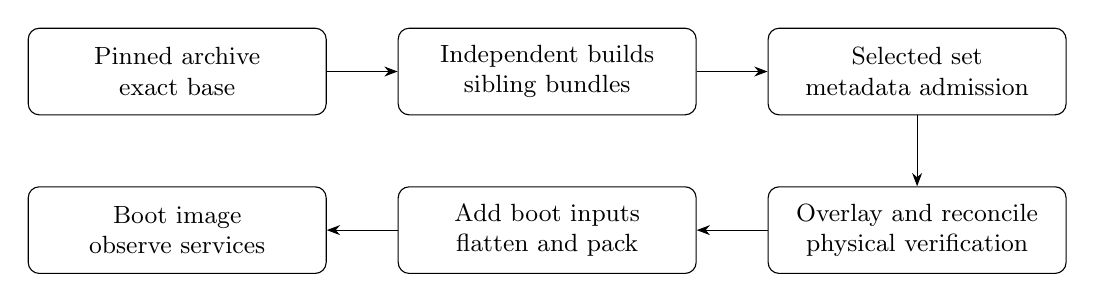
\begin{tikzpicture}[node distance=9mm and 9mm, box/.style={draw,rounded corners,align=center,text width=3.55cm,minimum height=11mm,font=\small}, >={Stealth}]
\node[box] (base) {Pinned archive\\exact base};
\node[box,right=of base] (deltas) {Independent builds\\sibling bundles};
\node[box,right=of deltas] (admit) {Selected set\\metadata admission};
\node[box,below=of admit] (merge) {Overlay and reconcile\\physical verification};
\node[box,left=of merge] (pack) {Add boot inputs\\flatten and pack};
\node[box,left=of pack] (boot) {Boot image\\observe services};
\draw[->] (base)--(deltas);\draw[->] (deltas)--(admit);\draw[->] (admit)--(merge);\draw[->] (merge)--(pack);\draw[->] (pack)--(boot);
\end{tikzpicture}
\caption{Server-side construction and verification of a selected root. Schematic; no measured quantities are represented. Diagram prepared with tool H1.}
\label{fig:architecture}
\end{figure}

\section{Conflict taxonomy and policy}

The conflict taxonomy separates mechanisms by the action they require. Some overlaps are harmless; some states must be rejected; others should be prevented before the bytes are created; shared registries need reconciliation; runtime resource contention needs execution. The policies in the taxonomy distinguish the observed mechanisms.

\Cref{tab:taxonomy} summarizes the corresponding contract.
\begin{table}[tbp]
\centering\small
\begin{tabularx}{\textwidth}{@{}p{2.6cm}YY@{}}
\toprule
Class & Mechanism & Policy \\
\midrule
\num{1}. Benign overlap & Siblings contribute the same package at the same version. & Accept at the package level and measure duplication. \\
\num{2}. Version skew & Package versions or parent/snapshot/generation identities disagree. & Reject before mounting. \\
\num{3}. Declared conflict & \texttt{Conflicts} or \texttt{Breaks}, including resolved virtual names, forbids coexistence. & Reject through package-relation checking. \\
\num{4}. File collision & Different packages own one path without a sanctioned replacement or diversion. & Intersect ownership sidecars and reject unsanctioned overlap. \\
\num{5}. State divergence & Independent installations rewrite complete shared registries. & Merge records or regenerate derived state. \\
\num{6}. Implicit base upgrade & A delta upgrades a package inherited from base. & Upgrade base first at the pin and detect recurrence. \\
\num{7}. Identity collision & Numeric owners and account identities disagree across siblings. & Partition allocation windows, merge records, and audit owners. \\
\num{8}. Runtime resource conflict & Installed services compete for a runtime resource. & Observe at Tier \num{3}; the earlier tiers do not model actual resource acquisition. \\
\num{9}. Opaque directory erasure & A directory marker captured in one build hides another sibling's files. & Strip opaque markers under checked build preconditions; check visibility. \\
\bottomrule
\end{tabularx}
\caption{Conflict mechanisms and their composition policies. The classes describe mechanisms, not mutually exclusive set outcomes.}
\label{tab:taxonomy}
\end{table}


\subsection{Package compatibility and file ownership}

Class \num{1} treats matching package identity as benign overlap for admission; it does not prove that post-install generated bytes match. Class \num{2} detects incompatible package versions and composability preconditions. Class \num{3} evaluates declared relations, including virtual names. A provided capability is not intrinsically exclusive: two providers without an explicit conflict are not rejected merely for providing the same name.

Module-level requirements are checked separately from Debian package relations. A selected CUDA module can require a selected driver module and an acceptable module version even if each was built alone against base. A set missing its driver may become acceptable when that driver is added. This is why a pairwise rejection is not automatically a permanent exclusion edge for a larger set. The current admission census demonstrates that distinction.

Class \num{4} needs the path-ownership sidecars, because package metadata alone does not enumerate every collision. Ownership intersection followed by replacement and diversion analysis has a direct predecessor in EDOS/Mancoosi \autocite[\S~2.2.5]{treinen2008solving}. \texttt{Replaces} and diversions require special treatment, but a declaration allowing dpkg to overwrite a path during sequential installation does not by itself reproduce those semantics in a static overlay. ModFS uses a conservative admission policy; complete replacement and diversion behavior remains a limit to the generality of the result. A package-owned path index also cannot classify every inode attribute or unowned generated file.

\subsection{Shared state and numeric identities}

Class \num{5} requires a semantic result for each shared database. Merely exempting its path from a collision report stops a warning without preserving the records. The registry-specific operations below define what is combined and what is regenerated.

Class \num{7} also requires prevention. Package scripts in independent roots can allocate the same free number to different services. Once files are stored with that owner, merging names does not remap the inodes. Permanent allocation windows prevent ordinary builds from making the collision. Both allocator interfaces must be configured before installation, and account metadata and file-owner lists must be checked afterwards. Shared accounts supplied by base still require consistent identities. The final deployed allocation policy must also avoid reusing module IDs for future local users, an unresolved lifecycle concern.

\subsection{Context-sensitive filesystem and runtime effects}

Union-mount research already describes opaque-directory semantics and the sensitivity of deletion markers to layer order \autocite{pendry1995union}. Class \num{9} arose because a captured filesystem operation has meaning relative to its lower layers. During a build, an opaque marker can hide only base entries. During composition, the same marker can hide a sibling that was absent when it was created. In the motivating case, \texttt{pyyaml} hid the \texttt{pytools} numpy tree without two packages claiming the same file path. A successful representation round trip through SquashFS therefore did not prove the desired sibling semantics.

The current build policy strips opaque markers only for direct-base siblings and rejects upperdirs containing whiteouts, a conservative guard against a deleting module whose directory-replacement intent could be destroyed. The storage format's ability to preserve whiteouts is not a validated arbitrary-removal workflow. V7 checks the resulting visible paths but still leaves equal-size content substitution outside its predicate.

Class \num{8} was added after boots exposed a failure beyond the successful package and structural checks. It marks the runtime boundary: \texttt{apache2} and \texttt{nginx} can be metadata-compatible and structurally complete while both seek port \num{80}. Their actual startup outcome depends on scheduling. The existing Tier-1 and Tier-2 models cannot observe that race. A future policy could statically warn about known configured listeners, but would not turn an offline package or path check into an observation of resource acquisition. Runtime results are therefore recorded separately from structural success.

\section{Building against the exact parent}

The base builder uses \texttt{debootstrap}, then upgrades the base against the same snapshot pockets that sibling installations will see. This prevents a module from receiving newer base libraries merely because its \ac{APT} view includes updates absent from the initial bootstrap. The snapshot identity is in the archive URL so both bootstrap and subsequent \ac{APT} operations use the same archive view.

A sibling build mounts the exact parent \texttt{base.sqsh} read-only and uses it as the lower filesystem of an OverlayFS mount. Packages are installed into the merged view, with an upperdir capturing newly written files, copies of modified base files, and deletion markers. The builder compresses only that upperdir. The exact-parent requirement matters: a leftover unpacked \texttt{base.dir} could contain bytes different from the archive whose digest is recorded in the generation. The immutable archive therefore supplies the parent; a leftover unpacked build directory is insufficient.

Before \ac{APT} runs, both account allocators are redirected to the assigned window: \texttt{adduser.conf} controls \texttt{adduser --system}, and \texttt{login.defs} controls \texttt{useradd -r}. Both are needed because package scripts use both tools. The builder restores the original allocator configuration before squashing. Deleting a base file instead would leave a whiteout that hides the base policy during composition. The extractor later checks declared accounts and numeric owners of shipped files, because a file can borrow another module's \ac{UID} even when its own module never declared that account.

Build-only mounts and daemon-start suppression let maintainer scripts run in the target root without treating it as a booted machine. A \texttt{policy-rc.d} hook prevents service startup; apt/dpkg logs and transient caches are excluded; the base machine identity is cleared; and archive inode timestamps are pinned. Completion markers are written after successful work. These measures remove specific unwanted outputs, but do not erase a password-change date embedded in \texttt{/etc/shadow}, a generated database identifier, or a host-dependent post-install result. They must not be described as a proof of byte reproducibility.

The builder also removes \texttt{trusted.overlay.opaque} under the checked flat-sibling preconditions. Such a marker was created against the base but would later hide entries from a sibling that did not exist at build time. The storage representation preserves ordinary file whiteouts, but the current builder conservatively refuses an upperdir containing them before applying this opaque-marker policy. Thus representation support for deletion is not demonstrated support for building arbitrary deleting siblings. The evaluated pattern is additive; removals and directory replacement remain a separate validation problem.

\section{Bundle representation and integrity}

\subsection{Artefact, manifest, and sidecar}

Each module consists of \texttt{<name>.sqsh}, \texttt{<name>.json}, and \texttt{<name>.files.json.zst}. The manifest is small enough for routine admission; the sidecar supplies per-path ownership when Class \num{4} needs it; physical composition mounts the archive. Thus Tier \num{1} avoids mounts and root privileges, although it does consume the relevant sidecars as well as manifests. It does not rehash all SquashFS bytes on every metadata decision: artefact consumption and re-derivation have their own checks.

\Cref{tab:manifest} summarizes the corresponding contract.
\begin{table}[tbp]
\centering\small
\begin{tabularx}{\textwidth}{@{}p{2.6cm}Y@{}}
\toprule
Manifest group & Fields and meaning \\
\midrule
Identity & \texttt{schema}, \texttt{module}, \texttt{version}, \texttt{parent}, \texttt{snapshot}, \texttt{suite}, \texttt{arch}, \texttt{built}, \texttt{generation}. \\
Installation & \texttt{requested}, contribution \texttt{packages}, and \texttt{removed}; each package retains its version and raw Debian relations. \\
Module policy & \texttt{requires}, \texttt{conflicts}, \texttt{provides}. \\
Identity and service observations & \texttt{uid\_range}, \texttt{accounts}, \texttt{identity\_audit}, \texttt{units}. \\
Artefact identity & \texttt{artifact.file}, \texttt{artifact.bytes}, \texttt{artifact.sha256}. \\
Integrity policy & \texttt{binding}, including required field coverage, source, and digests. \\
\bottomrule
\end{tabularx}
\caption{Responsibilities of the module manifest. Requested packages describe intent; extracted contributions describe the stored installation.}
\label{tab:manifest}
\end{table}


The sealed field set is explicit; ancillary metadata is not assumed to be covered merely because it appears in the document.

A module records only package contributions that differ from its parent, plus removals. Consumers reconstruct an effective package map from the base and contributions. If two selected sources offer incompatible versions, admission rejects the set before a map overwrite could conceal the disagreement. Package relations and module relations remain distinct: the latter require a selected module name or provided capability at an acceptable module version. Multiple providers of one capability are not automatically rejected unless an explicit conflict expresses that policy; provider cardinality is not represented.

The sidecar maps paths to owning package names and records diversions. Extraction operates on the stored module and parent artefacts so excluded build scratch cannot be mistaken for shipped content. This also lets the build tree be discarded. A sealed manifest can still describe the wrong \emph{requested specification} if no one compares the spec with the installation; \texttt{jq}'s earlier missing \texttt{moreutils} is the project's concrete example. Bundle consistency and fulfilment of operator intent are distinct conditions.

\subsection{What each digest proves}

\Cref{tab:digests} summarizes the corresponding contract.
\begin{table}[tbp]
\centering\small
\begin{tabularx}{\textwidth}{@{}p{2.6cm}YY@{}}
\toprule
Commitment & Bytes or fields covered & Consumer obligation \\
\midrule
Artefact digest & The exact \texttt{.sqsh} bytes, named by \texttt{artifact.sha256} and repeated in \texttt{binding.artifact\_sha256}. & Check agreement of the recorded fields and hash the actual archive when consuming its bytes. \\
Sidecar digest & \textbf{Decompressed \ac{JSON} bytes} from \texttt{.files.json.zst}. & Decompress, verify \texttt{binding.sidecar\_sha256}, then parse and use ownership data. \\
Field digest & Canonical \ac{JSON} of the required, named manifest fields. & Require the complete field list and presence of its members, then recompute \texttt{binding.fields\_sha256}. \\
\bottomrule
\end{tabularx}
\caption{Integrity contracts for a filesystem bundle. Each consumer must require the appropriate commitment before using its content.}
\label{tab:digests}
\end{table}


Changing the zstd encoding without changing its decompressed \ac{JSON} is outside the sidecar digest's scope.

The field digest includes the \texttt{artifact} record and \texttt{generation}. The field list is required by the consumer, not negotiated by the document being checked. Otherwise a shortened document could announce a shorter list and pass its own hash. The sidecar digest is required separately because the \texttt{binding} object is not part of the field payload. This is a schema-policy issue, not an inherent cryptographic rule that a sidecar digest could never itself be covered by another digest.

The binding verifier mounts artefacts and re-derives metadata, which is stronger than checking that a document's hashes agree internally. Even re-derivation does not establish the identity of a trusted publisher. Someone able to replace the whole bundle and reseal it can create a consistent different bundle. Signing and an external trust root are outside scope.

A generation consists of snapshot, suite, architecture, and exact base digest, together with an identifier derived from those values. Module specifications are deliberately absent: a specification may change within one generation. A metadata refresh preserves the recorded generation rather than relabelling old bytes as children of the current base. Adoption for legacy artefacts is an explicit assertion about their origin, not reconstruction of missing historical proof.

\section{Registry reconciliation}

The composer mounts each selected SquashFS layer and overlays a writable reconciliation layer above them. It supplies the reconciler with layer roots in the intended precedence order. The reconciler writes parsed registry results into the top layer, then the native tools regenerate derived state. Relative lowerdir paths keep mount-option length manageable at high N. Mount creation, reconciliation, regeneration, and teardown must all preserve an observable failure rather than allowing partial scratch state to become a publishable result.

\subsection{Package status and installation marks}

\texttt{dpkg/status} uses blank-line-separated stanzas. The format-level identity is package plus architecture, and different versions of the same effective package are incompatible. The current implementation, in the documented single-architecture scope, indexes status by package name. Consequently it should not be presented as a general multiarch union; an architecture-aware key is a required extension for that claim. Repeated installed stanzas at the same version retain a selected source stanza, while version disagreement contributes an error. Fields outside the compared version can still depend on the selected layer.

\texttt{extended\_states} also uses stanzas, but its semantics differ. \ac{APT} generally records automatic installation positively; manual installation can be represented by the \textbf{absence} of an automatic stanza. Combining only explicit entries would miss a sibling's manual request. The reconciler considers the installed package records together with automatic marks, lets manual intent dominate, and inherits base marks when a delta has no replacement file. An empty output can therefore be necessary to clear a top layer's obsolete automatic flags. This is not ordinary last-layer precedence.

\subsection{Alternatives and diversions}

An alternatives registry is positional: mode, generic link, slave-link definitions, then candidate paths, priorities, and slave targets. It must be parsed with that structure. \texttt{vim} offers \path{/usr/bin/vim.basic} at priority \num{30} and \texttt{emacs} offers \texttt{/usr/bin/emacs} at priority \num{0}; retaining both candidates and running automatic selection chooses vim. If layers assign different priorities to the \emph{same} candidate, the merger reports a conflict. It may retain the higher priority in the scratch output, but its nonzero result means that tree is not accepted. A diagnostic choice is not successful conflict resolution.

A diversion is a consecutive triple: original path, diverted path, and responsible package. Malformed or partial triples must fail rather than silently disappearing. A diversion is identified semantically by its original path. The present diversion parser deduplicates whole triples; it does not independently reject different triples sharing the same original path. Malformed-record rejection does not establish complete conflicting-diversion arbitration. The reference key and implementation behavior therefore differ, limiting the claimed scope.

\subsection{Accounts and debconf}

The account group comprises \texttt{passwd}, \texttt{group}, \texttt{shadow}, \texttt{gshadow}, \texttt{subuid}, and \texttt{subgid}. Their record shapes are centralized in a shared account-format schema; names identify the ordinary account records, while subordinate ranges are retained as whole-line sets. Numeric \ac{UID}, \ac{GID}, and primary-group disagreement is an error. Group and gshadow membership is unioned as sets rather than overwritten. Other fields follow the declared highest-layer policy, and sensitive modes and ownership are preserved. Disjoint allocation windows prevent ordinary numeric collisions, but do not remove the need for this record union.

Debconf's \texttt{config.dat}, \texttt{templates.dat}, and \texttt{passwords.dat} contain records keyed by \texttt{Name}. \texttt{Owners} is a set, so overlapping owners are deduplicated; continuation fields in templates must survive parsing. Conflicting values or other incompatible shared fields are reported, and \texttt{passwords.dat} retains its sensitive attributes. Missing record keys are errors. The parser cannot legitimately call a merge successful merely because it recognized a subset of the source.

The reconciler accumulates problems and returns failure even if it has already written diagnostic output to the scratch tree. Its caller must discard a failed composition. Tested order reversals preserve semantic record sets for the documented examples, but record order and bytes differ, and conflicting highest-layer fields do not acquire general order independence from this mechanism.

\subsection{Derived state and verification coverage}

\texttt{/etc/alternatives/*} is regenerated by \texttt{update-alternatives --auto} from the merged candidates. \texttt{/etc/ld.so.cache} is regenerated by \texttt{ldconfig} from the composed library tree. These are the last two of the eight registry groups. They are functions of the merged inputs, so unioning their old outputs is inappropriate. Failure of either native tool is a failed composition.

V2 checks package status, V3 alternatives, V4 the linker result, V6 accounts, and V8 debconf. V5 asks dpkg to audit its view, while V7 checks path visibility and selected file properties. This coverage does not give every registry an equally strong independent oracle: diversions and extended states do not have dedicated V-numbered semantic checks in the generated list. Trigger registrations also remain outside the handled registry set. These limits matter when interpreting a clean V1--V8 row.

\section{How the registry inventory was established}

The inventory grew through compositions whose visible behavior disagreed with their apparent package state. Lost package records motivated status reconciliation. A survey of paths shared by independent upperdirs exposed alternatives, diversions, and automatic-installation marks; inspecting library lookup exposed the derived cache. Account auditing revealed that unique numeric allocations still needed a union of account records. Enumerating shared unowned files then exposed configuration databases whose answers had disappeared beneath a later layer.

This supplies a repeatable discovery method: intersect the files present in multiple upperdirs and remove package-owned paths using the ownership inventory. The remaining shared files are candidates for semantic interpretation. They are not automatically interchangeable registries, and the survey does not prove complete coverage of every maintainer-script effect. Trigger registrations, for example, remain outside the implemented merge groups. New package families should prompt another survey, not an assumption that the existing list is universal.

\section{From admitted sets to a running image}

A requested plan maps layer counts to sample counts. The sampler combines declared requirements with exclusions learned from Tier-1 observations. It first explains a pair rejection that a later provider could satisfy; only irreducible exclusions belong in the pair-conflict model. Otherwise \texttt{fake-cuda} would be systematically excluded from high-layer sets despite belonging to an admissible set with its driver.

When the admissible space or its complement can be enumerated, \texttt{exact} mode samples uniformly from it and reports its cardinality. For larger spaces, \texttt{sampled} mode uses a seeded, closure-aware greedy construction and is reproducible without being uniform. Every proposal still goes through the admission checker. Refused proposals are evidence of model/checker disagreement, not observations to drop. The plan, seed, mode, attempted sets, and module coverage are needed to interpret a sweep; aggregate timing means alone cannot recover them.

Boot construction begins with bundle validation and admission. An explicit known-negative run may bypass the ordinary admission requirement for a stated experiment, but must not be labelled admitted. The same reconciliation mechanism then assembles the selected root. The packing stage adds a bootable kernel image, creates \ac{GPT}/\ac{EFI} and ext4 filesystems, copies the composed tree with numeric identities and attributes, and writes the boot configuration. Siblings do not contain the boot kernel image, although the driver sibling does contain kernel module objects; calling every sibling a purely userspace delta would conceal that \ac{ABI} dependency.

The guest harness records systemd state, foreign pending jobs, failed units, package audit, per-module probes, and listeners through serial markers. Its wait must exclude its own job, or the observer prevents the steady state it is waiting for. Probe observations prefixed for the harness are retained even on success. Partition devices must be usable before filesystem creation, and the disk must be sized for the actual root contents. These details determine whether the experiment tests the composed system or only a failure in its apparatus.

The bundle retains the serial log, verdict, run identity, and resolved kernel information. Recording a kernel digest establishes which boot input was used; it does not by itself make the whole build reproducible. Old bundles remain immutable, while later evidence generation assesses their currency against the artefact inventory. Freshness checks use recorded identities and rebuild times. A freshness label does not constitute new content verification of every old run.

\section{Verification and trust boundaries}

The checker must declare what it has observed. Missing sidecars or malformed nested ownership fields cannot be treated as an empty, clean set of paths or owners. Where the checker returns \texttt{ACCEPT WITH WARNINGS}, that is weaker than fully checked acceptance. A negative control is likewise specific: an old-snapshot control exercises composability rejection, but does not establish that every account or debconf predicate is effective. Adversarial tests target the individual observation boundaries.

Trusted inputs are another design assumption. Packing and reconciliation invoke tools from composed roots with host-side privileges before the VM boundary. Bundle digests detect drift and internal inconsistency; they do not isolate hostile package code. The prototype therefore concerns a controlled build catalogue, not a service safely composing arbitrary untrusted customer artefacts. This limit follows from where code executes, independently of whether its files have consistent hashes.

\section{Updates, publication, and rollback}

An intra-generation specification update rebuilds the affected sibling against the unchanged exact base, refreshes its manifest and sidecar, and repeats binding, admission, and relevant later checks. Rebuilding at a fixed snapshot cannot obtain a security version absent from that archive. A pin move instead builds a new base and all siblings in an isolated generation. The selected generation must be exposed coherently; the current implementation has no transactional remote publisher providing that atomicity.

Build work and transfer opportunity are separate. A byte-identical artefact could be reused from a content-addressed cache, while a changed hash requires the whole new archive under the current reporting model. An unchanged file size is not sufficient for reuse. No implemented remote client or block-difference protocol turns these byte comparisons into a measured network result.

The selected root is flattened into an ordinary image for delivery. Rollback means redeploying a retained complete bootable image and its configuration identity, or retaining every input needed to reconstruct that image. Base and deltas alone omit the packing-time kernel, initramfs, bootloader, and configuration. Operating-system rollback also does not undo application data or schema changes. These boundaries determine what \cref{ch:analysis} measures and why repository savings cannot be presented as per-node update or rollback performance.


\chapter{Analysis}
\label{ch:analysis}

The evaluation follows the system from selected package metadata to a running machine. Compatibility requires an admission census and physical compositions; storage requires an artefact inventory and a comparison model; verification requires examining both successful observations and counterexamples to the checkers. Each experiment answers a different part of the research questions. The source files, digests, generation dates, and historical evidence identities are retained in \cref{app:provenance}.

\section{Populations and experimental scope}

Throughout this chapter, $N$ counts sibling deltas, excluding the shared base. The current catalogue contains \dref{/catalogue/total} entries: \dref{/catalogue/real} real workloads, \dref{/catalogue/synthetic} synthetic modules, and \dref{/catalogue/control} deliberately incompatible control. It was assembled to exercise conflict mechanisms, rather than sampled from a deployment population. Exhaustive admission covers pairs and triples; physical composition samples larger sets and covers \dref{/catalogue/covered} distinct ordinary deltas. That coverage count excludes the control and does not identify a separate catalogue generation.

The refreshed physical sweep and current storage inventory supersede the earlier physical measurements. Historical boot bundles remain a separate population: a new composition sweep does not retroactively boot its artefacts. A selected bundle's freshness identifies its relationship to rebuilt inputs, rather than certifying all current combinations. The evaluation therefore distinguishes current structural observations from historical demonstrations of runtime mechanisms.

Sampling also limits inference. Small enumerable admissible spaces permit uniform draws; the larger-space seeded heuristic is reproducible without being uniform. Every proposal must still pass authoritative admission. The aggregate evidence does not retain enough sampling or timing detail to estimate a population-wide failure probability, controlled cache-state effect, or uncertainty interval. Its fitted durations describe the measured sweep.

\section{Static admission: coverage and its limits}

\Cref{tab:admission} reports the exhaustive census. The larger rejected share among triples can arise because adding a module introduces further incompatible relationships. It must not be interpreted as a general probability that an arbitrary user-selected system will fail: the catalogue deliberately includes adversarial cases and an incompatible control.

\begin{table}[tbp]
\centering
\begin{tabular}{rrrr}
\toprule
$N$ & Sets & ACCEPT & REJECT \\
\midrule
\num{2} & \dref{/tier1/totals/2/combinations} & \dref{/tier1/totals/2/accept} & \dref{/tier1/totals/2/reject} \\
\num{3} & \dref{/tier1/totals/3/combinations} & \dref{/tier1/totals/3/accept} & \dref{/tier1/totals/3/reject} \\
\bottomrule
\end{tabular}
\caption{Exhaustive admission of pairs and triples from the \dref{/catalogue/total}-module catalogue, including the incompatible control.}
\label{tab:admission}
\end{table}

\Cref{tab:causes} separates rejection conditions. Module relations include unsatisfied requirements as well as declared incompatibilities; a missing CUDA driver and mutually incompatible mail providers are therefore different mechanisms in the same column. Columns overlap because one selected set can violate several conditions. Zero observations for file collision, identity collision, and implicit base upgrade describe the constructed catalogue and implemented predicates. They do not prove that arbitrary installations cannot create those conflicts.

\begin{table}[tbp]
\centering\small
\begin{tabular}{lrr}
\toprule
Condition & Pairs & Triples \\
\midrule
Version skew & \dref{/tier1/classes/2/version-skew} & \dref{/tier1/classes/3/version-skew} \\
Declared conflict & \dref{/tier1/classes/2/declared-conflict} & \dref{/tier1/classes/3/declared-conflict} \\
File collision & \dref{/tier1/classes/2/file-collision} & \dref{/tier1/classes/3/file-collision} \\
Identity collision & \dref{/tier1/classes/2/identity-collision} & \dref{/tier1/classes/3/identity-collision} \\
Module relation & \dref{/tier1/classes/2/module-relation} & \dref{/tier1/classes/3/module-relation} \\
Implicit base upgrade & \dref{/tier1/classes/2/base-drift} & \dref{/tier1/classes/3/base-drift} \\
Not composable & \dref{/tier1/classes/2/not-composable} & \dref{/tier1/classes/3/not-composable} \\
\bottomrule
\end{tabular}
\caption{Overlapping rejection conditions for the \dref{/catalogue/total}-module census. These counts are not a partition of rejected sets.}
\label{tab:causes}
\end{table}

The old-snapshot control is refused with every ordinary sibling. It accounts for \dref{/tier1/classes/2/not-composable} flagged pairs and \dref{/tier1/classes/3/not-composable} flagged triples. This rules out an all-accept checker but exercises one particular composability condition. Positive controls for other predicates must construct their own violating inputs.

Admission is not monotone under set extension. Among \dref{/tier1/crosscheck/3/sets-containing-rejecting-pair} triples containing a rejecting pair, \dref{/tier1/crosscheck/3/accept-despite-rejecting-pair} are accepted. The accepted exceptions concern module relations: adding a missing provider can complete a requirement. Adding a provider does not repair a genuine incompatibility between packages already present. The census contains no rejected triple unexplained by an inner rejecting pair, but this internal cross-check remains an observation of the checker rather than an independent proof of physical correctness.

Benign overlap occurs in \dref{/tier1/measured/2/sets-with-benign-overlap} pairs and \dref{/tier1/measured/3/sets-with-benign-overlap} triples. Sanctioned replacement or diversion suppresses collisions in \dref{/tier1/measured/2/sets-with-suppressed-collision} pair and \dref{/tier1/measured/3/sets-with-suppressed-collision} triples. These are sets with a condition, not necessarily accepted sets: another predicate can still reject them. The observations show that overlap is classified rather than universally forbidden; they do not measure duplicated bytes.

\section{Physical composition and the cost of observation}

\subsection{Sampled systems and recorded predicates}

All \dref{/tier2/current/compose/n} sampled compositions pass the recorded checks. \Cref{tab:physical} gives their distribution and mean durations. Package counts vary at fixed $N$, because a sibling can contribute a thin utility or a substantial dependency closure. At the upper end only \dref{/timing/38/samples} samples contribute to the mean. Independently rounded phase means need not add exactly to the displayed composition mean.

\begin{table}[tbp]\centering\small
\begin{tabular}{rrrrrrr}
\toprule $N$ & Samples & Packages & Mount & Reconcile & Compose & Verify \\
\midrule
\dref{/timing/2/n} & \dref{/timing/2/samples} & \numrange{\drefvalueof{/timing/2/packages-min}}{\drefvalueof{/timing/2/packages-max}} & \dref{/timing/2/mount-ms-mean} & \dref{/timing/2/reconcile-ms-mean} & \dref{/timing/2/total-ms-mean} & \dref{/timing/2/verify-ms-mean} \\
\dref{/timing/3/n} & \dref{/timing/3/samples} & \numrange{\drefvalueof{/timing/3/packages-min}}{\drefvalueof{/timing/3/packages-max}} & \dref{/timing/3/mount-ms-mean} & \dref{/timing/3/reconcile-ms-mean} & \dref{/timing/3/total-ms-mean} & \dref{/timing/3/verify-ms-mean} \\
\dref{/timing/5/n} & \dref{/timing/5/samples} & \numrange{\drefvalueof{/timing/5/packages-min}}{\drefvalueof{/timing/5/packages-max}} & \dref{/timing/5/mount-ms-mean} & \dref{/timing/5/reconcile-ms-mean} & \dref{/timing/5/total-ms-mean} & \dref{/timing/5/verify-ms-mean} \\
\dref{/timing/10/n} & \dref{/timing/10/samples} & \numrange{\drefvalueof{/timing/10/packages-min}}{\drefvalueof{/timing/10/packages-max}} & \dref{/timing/10/mount-ms-mean} & \dref{/timing/10/reconcile-ms-mean} & \dref{/timing/10/total-ms-mean} & \dref{/timing/10/verify-ms-mean} \\
\dref{/timing/15/n} & \dref{/timing/15/samples} & \numrange{\drefvalueof{/timing/15/packages-min}}{\drefvalueof{/timing/15/packages-max}} & \dref{/timing/15/mount-ms-mean} & \dref{/timing/15/reconcile-ms-mean} & \dref{/timing/15/total-ms-mean} & \dref{/timing/15/verify-ms-mean} \\
\dref{/timing/20/n} & \dref{/timing/20/samples} & \numrange{\drefvalueof{/timing/20/packages-min}}{\drefvalueof{/timing/20/packages-max}} & \dref{/timing/20/mount-ms-mean} & \dref{/timing/20/reconcile-ms-mean} & \dref{/timing/20/total-ms-mean} & \dref{/timing/20/verify-ms-mean} \\
\dref{/timing/25/n} & \dref{/timing/25/samples} & \numrange{\drefvalueof{/timing/25/packages-min}}{\drefvalueof{/timing/25/packages-max}} & \dref{/timing/25/mount-ms-mean} & \dref{/timing/25/reconcile-ms-mean} & \dref{/timing/25/total-ms-mean} & \dref{/timing/25/verify-ms-mean} \\
\dref{/timing/27/n} & \dref{/timing/27/samples} & \numrange{\drefvalueof{/timing/27/packages-min}}{\drefvalueof{/timing/27/packages-max}} & \dref{/timing/27/mount-ms-mean} & \dref{/timing/27/reconcile-ms-mean} & \dref{/timing/27/total-ms-mean} & \dref{/timing/27/verify-ms-mean} \\
\dref{/timing/30/n} & \dref{/timing/30/samples} & \numrange{\drefvalueof{/timing/30/packages-min}}{\drefvalueof{/timing/30/packages-max}} & \dref{/timing/30/mount-ms-mean} & \dref{/timing/30/reconcile-ms-mean} & \dref{/timing/30/total-ms-mean} & \dref{/timing/30/verify-ms-mean} \\
\dref{/timing/33/n} & \dref{/timing/33/samples} & \numrange{\drefvalueof{/timing/33/packages-min}}{\drefvalueof{/timing/33/packages-max}} & \dref{/timing/33/mount-ms-mean} & \dref{/timing/33/reconcile-ms-mean} & \dref{/timing/33/total-ms-mean} & \dref{/timing/33/verify-ms-mean} \\
\dref{/timing/35/n} & \dref{/timing/35/samples} & \numrange{\drefvalueof{/timing/35/packages-min}}{\drefvalueof{/timing/35/packages-max}} & \dref{/timing/35/mount-ms-mean} & \dref{/timing/35/reconcile-ms-mean} & \dref{/timing/35/total-ms-mean} & \dref{/timing/35/verify-ms-mean} \\
\dref{/timing/38/n} & \dref{/timing/38/samples} & \numrange{\drefvalueof{/timing/38/packages-min}}{\drefvalueof{/timing/38/packages-max}} & \dref{/timing/38/mount-ms-mean} & \dref{/timing/38/reconcile-ms-mean} & \dref{/timing/38/total-ms-mean} & \dref{/timing/38/verify-ms-mean} \\
\bottomrule\end{tabular}
\caption{Physical sample from the \dref{/catalogue/total}-module catalogue; \dref{/catalogue/covered} distinct ordinary deltas are covered. $N$ excludes base. Durations are mean milliseconds; package columns give observed ranges.}\label{tab:physical}
\end{table}


The clean result means that each implemented predicate accepted each sampled tree. V1 is inferred from a positive reconciliation duration; it is weaker than a separately captured exit status. V2 checks installed package names and versions, V3 retained alternatives candidates, V4 the expected union of library \acp{SONAME} in the regenerated cache, and V5 the package-manager audit. V6 checks account records and membership, V7 path visibility and selected kind, size, and link properties, and V8 debconf records. Every column records \dref{/checks/V1/passing} of \dref{/checks/V1/total} passing rows.

These predicates differ in strength. A regenerated linker cache need not match a layer cache byte for byte to contain the expected \acp{SONAME}. Conversely, a regular file with different bytes but the same size can satisfy V7. Registry paths exempted from ordinary visibility checks need their own semantic assertions. Passing the sweep therefore establishes neither general filesystem equivalence nor service coexistence. The later counterexamples concern the observation boundary, not a contradiction in the reported clean rows.

\subsection{Scaling within the measured range}

\Cref{tab:fits,fig:timing} show approximately linear phase costs over the tested layer counts. Composition comprises mounting and reconciliation; verification is timed separately. Mounting more layers adds mount and namespace work, while reconciliation processes their package and registry state. Those mechanisms are consistent with the trend, but $N$ also covaries with package and record counts. The regression alone does not isolate their individual costs or prove that payload size has no effect.

\begin{table}[tbp]
\centering
\begin{tabular}{lrrr}
\toprule
Phase & $a$ (\si{\milli\second}) & $b$ (\si{\milli\second}/module) & $R^2$ \\
\midrule
Mount & \dref{/tier2/current/mount/intercept-ms} & \dref{/tier2/current/mount/slope-ms-per-module} & \dref{/tier2/current/mount/r2} \\
Reconcile & \dref{/tier2/current/reconcile/intercept-ms} & \dref{/tier2/current/reconcile/slope-ms-per-module} & \dref{/tier2/current/reconcile/r2} \\
Compose & \dref{/tier2/current/compose/intercept-ms} & \dref{/tier2/current/compose/slope-ms-per-module} & \dref{/tier2/current/compose/r2} \\
Verify & \dref{/tier2/current/verify/intercept-ms} & \dref{/tier2/current/verify/slope-ms-per-module} & \dref{/tier2/current/verify/r2} \\
\bottomrule
\end{tabular}
\caption{Fits $t(N)=a+bN$ over \dref{/tier2/current/compose/n} physical compositions covering \dref{/catalogue/covered} ordinary deltas of the \dref{/catalogue/total}-module catalogue. $N$ excludes base.}
\label{tab:fits}
\end{table}

% H1: plotting code prepared with AI assistance (see app:aids)
\begin{figure}[tbp]\centering
\begin{tikzpicture}
\begin{axis}[width=.94\textwidth,height=6.7cm,xlabel={Sibling deltas $N$ (base excluded)},ylabel={Duration (\si{\milli\second})},xmin=0,xmax=40,ymin=0,grid=major,legend pos=north west,legend style={font=\small}]
\addplot[only marks,blue,mark=*] coordinates {(\drefvalueof{/timing/2/n},\drefvalueof{/timing/2/total-ms-mean}) (\drefvalueof{/timing/3/n},\drefvalueof{/timing/3/total-ms-mean}) (\drefvalueof{/timing/5/n},\drefvalueof{/timing/5/total-ms-mean}) (\drefvalueof{/timing/10/n},\drefvalueof{/timing/10/total-ms-mean}) (\drefvalueof{/timing/15/n},\drefvalueof{/timing/15/total-ms-mean}) (\drefvalueof{/timing/20/n},\drefvalueof{/timing/20/total-ms-mean}) (\drefvalueof{/timing/25/n},\drefvalueof{/timing/25/total-ms-mean}) (\drefvalueof{/timing/27/n},\drefvalueof{/timing/27/total-ms-mean}) (\drefvalueof{/timing/30/n},\drefvalueof{/timing/30/total-ms-mean}) (\drefvalueof{/timing/33/n},\drefvalueof{/timing/33/total-ms-mean}) (\drefvalueof{/timing/35/n},\drefvalueof{/timing/35/total-ms-mean}) (\drefvalueof{/timing/38/n},\drefvalueof{/timing/38/total-ms-mean})};
\addlegendentry{Compose mean}
\addplot[blue,domain=2:38,no marks,dashed] {\drefvalueof{/tier2/current/compose/intercept-ms}+\drefvalueof{/tier2/current/compose/slope-ms-per-module}*x};
\addlegendentry{Compose fit}
\addplot[only marks,orange,mark=square*] coordinates {(\drefvalueof{/timing/2/n},\drefvalueof{/timing/2/verify-ms-mean}) (\drefvalueof{/timing/3/n},\drefvalueof{/timing/3/verify-ms-mean}) (\drefvalueof{/timing/5/n},\drefvalueof{/timing/5/verify-ms-mean}) (\drefvalueof{/timing/10/n},\drefvalueof{/timing/10/verify-ms-mean}) (\drefvalueof{/timing/15/n},\drefvalueof{/timing/15/verify-ms-mean}) (\drefvalueof{/timing/20/n},\drefvalueof{/timing/20/verify-ms-mean}) (\drefvalueof{/timing/25/n},\drefvalueof{/timing/25/verify-ms-mean}) (\drefvalueof{/timing/27/n},\drefvalueof{/timing/27/verify-ms-mean}) (\drefvalueof{/timing/30/n},\drefvalueof{/timing/30/verify-ms-mean}) (\drefvalueof{/timing/33/n},\drefvalueof{/timing/33/verify-ms-mean}) (\drefvalueof{/timing/35/n},\drefvalueof{/timing/35/verify-ms-mean}) (\drefvalueof{/timing/38/n},\drefvalueof{/timing/38/verify-ms-mean})};
\addlegendentry{Verify mean}
\addplot[orange,domain=2:38,no marks,dashed] {\drefvalueof{/tier2/current/verify/intercept-ms}+\drefvalueof{/tier2/current/verify/slope-ms-per-module}*x};
\addlegendentry{Verify fit}
\end{axis}\end{tikzpicture}
\caption{Physical phase means and fits for the \dref{/catalogue/total}-module catalogue (\dref{/catalogue/covered} ordinary deltas covered). Sample counts appear in \cref{tab:physical}; the fit uses all \dref{/tier2/current/compose/n} rows. Aggregate summaries supply no dispersion estimates, so no uncertainty band is inferred.}\label{fig:timing}
\end{figure}


Adding the composition and verification fits from the same sample gives
\begin{equation}
t_{\mathrm{compose+verify}}(N)=
\bigl(\dref{/tier2/combined/intercept-ms}+\dref{/tier2/combined/slope-ms}N\bigr)\,\si{\milli\second}.
\label{eq:combined-time}
\end{equation}
This sum covers the measured phases, without automatically including planning, setup, or teardown outside their timers. No combined $R^2$ is supplied: separate coefficients of determination cannot be added. At $N=\dref{/timing/38/n}$, the observed means are \dSI{/timing/38/total-ms-mean}{\milli\second} for composition and \dSI{/timing/38/verify-ms-mean}{\milli\second} for verification. Reporting only the composition mean would omit a substantial part of the structural observation cost.

The previous sweep fitted composition as $\dref{/tier2/previous/compose/intercept-ms}+\dref{/tier2/previous/compose/slope-ms-per-module}N$ milliseconds. The current slope differs by \dSI{/comparison/slope-change-pct}{\percent}, while the intercept falls by \dSI{/comparison/intercept-change-pct}{\percent}. This asymmetry suggests that repeated per-layer work is more stable than fixed overhead in these observations. It does not identify the slope as an intrinsic constant of the method or the intercept solely as a machine property: artefacts, workload mix, and checking context changed together. Verification's slope also changes from \dref{/tier2/previous/verify/slope-ms-per-module} to \dref{/tier2/current/verify/slope-ms-per-module} milliseconds per module. The evidence supports descriptive agreement for composition, not a controlled causal comparison or portability guarantee.

\section{Repository storage and workload dependence}

\subsection{The comparison being measured}

Let $B$ denote compressed base size and $d_i$ the compressed sibling sizes. Retaining a library of independent single-module variants is modelled as
\begin{equation}
S_{\mathrm{mono}}=NB+\sum_i d_i,\qquad
S_{\mathrm{ModFS}}=B+\sum_i d_i,\qquad
R=\frac{S_{\mathrm{mono}}}{S_{\mathrm{ModFS}}}.
\label{eq:storage}
\end{equation}
The base is \dSI{/storage/base-mb}{\mega\byte}; units are decimal throughout. Both sides concern compressed root-filesystem artefacts, excluding disk envelopes, kernels, and firmware partitions. The model neither enumerates every possible multi-module image nor compares against a repository with cross-image deduplication. It also does not measure bytes transferred to a node.

\Cref{tab:storage,fig:storage} show the cohort dependence. The small cohort benefits because repeated base copies would dominate its thin deltas. Large compilers, runtimes, and database closures retain substantial unique content, reducing the ratio. The whole-catalogue result reflects that mixture; it is not a universal storage factor for modular images.

\begin{table}[tbp]
\centering\small
\begin{tabular}{lrrrr}
\toprule
Cohort & $N$ & Stored (\si{\mega\byte}) & Model (\si{\mega\byte}) & Ratio \\
\midrule
Small adversarial & \dref{/storage/small/n} & \dref{/storage/small/stored-mb} & \dref{/storage/small/monolithic-mb} & \dref{/storage/small/ratio}$\times$ \\
Large realistic & \dref{/storage/large/n} & \dref{/storage/large/stored-mb} & \dref{/storage/large/monolithic-mb} & \dref{/storage/large/ratio}$\times$ \\
Whole catalogue & \dref{/storage/all/n} & \dref{/storage/all/stored-mb} & \dref{/storage/all/monolithic-mb} & \dref{/storage/all/ratio}$\times$ \\
\bottomrule
\end{tabular}
\caption{Compressed repository sizes for cohorts of the \dref{/catalogue/total}-module catalogue. Every monolithic value uses the additive model; independent builds calibrate it. Each cohort includes one shared base.}
\label{tab:storage}
\end{table}

\begin{figure}[tbp]\centering
\begin{tikzpicture}
\begin{axis}[ybar,bar width=15pt,width=.94\textwidth,height=6cm,ymin=0,ymax=4200,ylabel={Compressed size (\si{\mega\byte})},symbolic x coords={Small,Large,All},xtick=data,legend pos=north west,legend style={font=\small},scaled y ticks=false,ymajorgrids]
\addplot[fill=blue!50,draw=blue] coordinates {(Small,\drefvalueof{/storage/small/stored-mb}) (Large,\drefvalueof{/storage/large/stored-mb}) (All,\drefvalueof{/storage/all/stored-mb})};
\addlegendentry{Stored base and deltas}
\addplot[fill=orange!50,draw=orange] coordinates {(Small,\drefvalueof{/storage/small/monolithic-mb}) (Large,\drefvalueof{/storage/large/monolithic-mb}) (All,\drefvalueof{/storage/all/monolithic-mb})};
\addlegendentry{Modelled monoliths}
\end{axis}\end{tikzpicture}
\caption{Storage comparison for the \dref{/catalogue/total}-module catalogue: \dref{/storage/small/n} small and \dref{/storage/large/n} large modules. Each cohort counts the base once in modular storage; cohort bars therefore must not be summed. Plot preparation assisted by H1.}\label{fig:storage}
\end{figure}


CUDA illustrates the large-payload effect: its delta is \dSI{/module/cuda-runtime/delta-mb}{\mega\byte}, with a modelled marginal saving of \dSI{/module/cuda-runtime/saving-pct}{\percent}. Marginal saving assumes that the server already holds the base; an isolated one-module repository stores base plus delta and receives no sharing benefit under this model. Excluding CUDA increases the catalogue ratio to \dref{/sensitivity/3/ratio}$\times$. Excluding the control and synthetic entries instead leaves \dref{/sensitivity/2/n} real workloads at \dref{/sensitivity/2/ratio}$\times$. These changes expose workload selection as part of the result.

Catalogue identity includes the requested workload, not only its name or entry count. A rebuilt utility module can grow when an omitted requested package is restored. Its old and new sizes then describe different installations even if both catalogues have the same number of entries. Bundle seals establish consistency between captured content and metadata, but an additional specification-to-installation comparison is needed to establish that the intended request was fulfilled. The storage comparison therefore uses the refreshed artefact inventory consistently and does not interpret a change between differently defined variants as an improvement in compression. This also limits transferring the cohort labels to future catalogues: adding a dependency-heavy workload can change the ratio without changing the sharing mechanism.

\subsection{Calibration and baseline equivalence}

\Cref{tab:calibration} compares the additive approximation with independently built monoliths. The model exceeds those measurements by \dSI{/calibration/pytools/model-error-pct}{\percent} to \dSI{/calibration/jq/model-error-pct}{\percent}. That baseline-size error biases the apparent benefit upward; it is not the same percentage-point error in every saving ratio. The headline numerator remains modelled for all catalogue entries, rather than mixing measured and modelled sizes.

\begin{table}[tbp]\centering\small
\begin{tabular}{lrrr}
\toprule Module & Measured (\si{\mega\byte}) & Model (\si{\mega\byte}) & Error (\si{\percent}) \\
\midrule
curl & \dref{/calibration/curl/measured-mb} & \dref{/calibration/curl/modelled-mb} & \dref{/calibration/curl/model-error-pct} \\
emacs & \dref{/calibration/emacs/measured-mb} & \dref{/calibration/emacs/modelled-mb} & \dref{/calibration/emacs/model-error-pct} \\
jq & \dref{/calibration/jq/measured-mb} & \dref{/calibration/jq/modelled-mb} & \dref{/calibration/jq/model-error-pct} \\
nc-traditional & \dref{/calibration/nc-traditional/measured-mb} & \dref{/calibration/nc-traditional/modelled-mb} & \dref{/calibration/nc-traditional/model-error-pct} \\
pytools & \dref{/calibration/pytools/measured-mb} & \dref{/calibration/pytools/modelled-mb} & \dref{/calibration/pytools/model-error-pct} \\
webserver & \dref{/calibration/webserver/measured-mb} & \dref{/calibration/webserver/modelled-mb} & \dref{/calibration/webserver/model-error-pct} \\
\bottomrule\end{tabular}
\caption{Independent monolithic calibration within the \dref{/catalogue/total}-module catalogue. Positive error means the additive model exceeds the measured monolith size.}\label{tab:calibration}
\end{table}


The calibration covers smaller deltas. Its largest is Emacs at \dSI{/module/emacs/delta-mb}{\mega\byte}, below the large cohort's smallest delta, MySQL at \dSI{/module/mysql/delta-mb}{\mega\byte}. It consequently supplies no measured error bound for CUDA or the other large monoliths. Their contribution dominates the uncertainty in the aggregate comparison.

The independent monolithic builder also uses a separate bootstrap path. It does not reproduce the base builder's full upgrade and machine-identity normalization. A recently rebuilt comparator can therefore be fresh without being input-equivalent. The observed small size discrepancies combine compression effects with possible construction differences. A matched baseline would hold package versions, generated state, and construction policy constant. The existing calibration supports a bounded approximation, rather than a controlled estimate of the compression penalty alone.

\subsection{Thin and fat bases}

A historical catalogue experiment explores moving shared dependencies into a larger base. If the base grows by $\Delta B$ and each delta shrinks by $s_m$, repository storage changes by
\begin{equation}
\Delta S_{\mathrm{repository}}=\Delta B-\sum_{m\in M}s_m.
\end{equation}
The retained historical model decreases from \dSI{/fatbase/thin}{\mega\byte} to \dSI{/fatbase/fat}{\mega\byte}, a derived \dSI{/fatbase/reduction-pct}{\percent}. This concerns a \dref{/fatbase/n}-module experiment, not the current whole-catalogue total. The base increment is \dSI{/fatbase/base-increment}{\mega\byte}, whereas the largest individual delta saving is \dSI{/fatbase/best-delta-saving}{\mega\byte}, for \ac{GCC}. No single-module selection offsets that increment under the experiment's additive layer model.

For a fleet whose node $k$ selects $A_k$, the analogous repeated-payload model is
\begin{equation}
\Delta F=K\Delta B-\sum_{k=1}^{K}\sum_{m\in A_k}s_m.
\end{equation}
This explains why a repository can benefit while a specialized node does not. It remains a model: flattening removes overwritten paths and changes compression, while caches and deployment protocols alter transfer costs. Summing independently compressed dependency sizes can also double-count shared content. Base selection therefore requires the fleet's workload distribution and measurements of its actual packed images; the repository result alone does not choose the best base for every node.

\section{Boot observations and runtime conflicts}

The retained history contains \dref{/boot/bundles} bundles: \dref{/boot/pass} PASS, \dref{/boot/fail} FAIL, \dref{/boot/broken} BROKEN, \dref{/boot/aborted} ABORTED, and \dref{/boot/no-result} without a result. These labels separate observed guest outcomes from missing observations or apparatus failures. They are not independent trials of one fixed system and must not be turned into a deployment success rate. Only the GPU pair's two bundles remain non-superseded, including one aborted attempt.

\Cref{tab:boots} retains the observations needed to interpret the runtime conflict. Each web server starts alone in its historical image. In both composed orders, nginx owns port \num{80} and the Apache unit fails despite passing package audit and both command probes. The selected service set introduces contention that the lower tiers did not model. Reversing filesystem order is not equivalent to controlling service scheduling, so the observations establish a conflict without proving a universal winner.

\begin{table}[tbp]\centering\small
\begin{tabularx}{\textwidth}{@{}Ylrl@{}}
\toprule Selected modules / order & Verdict & Time (\si{\second}) & Key observation \\
\midrule
nginx alone & PASS & \dref{/boot/run/11/duration-s} & nginx listener \\
Apache alone & PASS & \dref{/boot/run/14/duration-s} & Apache listener \\
nginx, Apache & FAIL & \dref{/boot/run/15/duration-s} & Apache failed \\
Apache, nginx & FAIL & \dref{/boot/run/16/duration-s} & Apache failed \\
MySQL, PostgreSQL & PASS & \dref{/boot/run/0/duration-s} & Both listeners \\
PostgreSQL, MySQL & PASS & \dref{/boot/run/4/duration-s} & Both listeners \\
Large selected set & FAIL & \dref{/boot/run/19/duration-s} & Apache failed \\
Driver, CUDA runtime & PASS & \dref{/boot/run/8/duration-s} & No GPU access \\
\bottomrule\end{tabularx}
\caption{Selected boot observations from the retained history, not a current exhaustive \dref{/catalogue/total}-module boot census. The large selected set has \dref{/boot/run/19/n} deltas. Only the displayed GPU pair remains non-superseded; its probes do not test hardware operation.}\label{tab:boots}
\end{table}


The high-layer runs likewise record progressively more passing probes, ultimately all selected probes, while the failed Apache unit persists. Evolving artefacts and harnesses prevent interpreting the sequence as repeated trials or a failure-rate improvement. Its useful conclusion is that a probe can demonstrate command availability while leaving service health untested. Database order reversals preserve working database probes and separate listeners; their recorded system state is still \texttt{starting}, which is weaker than a fully settled \texttt{running} state.

The current GPU-pair boot records successful probes and a running guest without access to GPU hardware. A separate userspace test used a provider's already installed driver. Neither observation demonstrates that the packaged kernel driver can operate a GPU. That claim requires matching hardware, the intended kernel \ac{ABI}, and the deployment's signing policy. A separate distribution-portability investigation must likewise retain its own artefact and measurement identity rather than supplementing this catalogue's results silently.

The \dref{/boot/completed} completed PASS/FAIL runs span \dSI{/boot/min-s}{\second} to \dSI{/boot/max-s}{\second}. Using \cref{eq:combined-time} only as a descriptive denominator, two-module boots take approximately \dref{/gap/2/min}--\dref{/gap/2/max} times the fitted physical phases; the historical \dref{/boot/run/19/n}-module boots take approximately \dref{/gap/36/min}--\dref{/gap/36/max} times as long. These are unmatched comparisons of the refreshed physical fit with historical boot runs. They indicate the scale of the observation cost, without isolating a speedup or a hardware-independent tier ratio. No admission-to-composition timing factor is inferred from the untraceable admission durations.

\section{What adversarial verification revealed}

The clean physical sweep did not discover every genuine defect. Directed fixtures exposed repeated accounts with inconsistent primary groups, duplicate membership retention, and incomplete diversion records silently discarded by the merger. Earlier successful rows had not observed those conditions. The precise conclusion is that Tier \num{2} did not reject these genuine defects until its checkers were taught to see them; it is not that composition never failed.

The findings fall into three qualitative groups. First, predicates can observe an insufficient property: matching package names without versions, exempting a rewritten registry without checking its records, or comparing file size without content. Second, the harness can alter or misobserve its subject: waiting for all jobs while counting its own job prevents the expected settled state, and successful version probes can conceal failed services. Third, evidence handling can misstate scope: a composition timer omits separately timed verification, a recent summary can omit sets, and a schema change can invalidate old manifests even when archive hashes still agree.

Each repair requires a counterexample and a positive control. A regression expecting rejection of malformed input verifies a different behavior from one expecting a semantic merge. A passing known-open fixture can intentionally confirm that a blind spot remains reproducible. Consequently, green test summaries and counts of documentation corrections cannot substitute for a deduplicated implementation-defect inventory or a completeness argument.

V7's equal-size substitution remains a concrete limitation. Hashing contested paths would strengthen content preservation, but only after defining the intended winning layer and legitimate exceptions for generated state, links, modes, and ownership. Shared parsers also create correlated errors: producer and checker can agree on the same mistaken interpretation. Independently constructed fixtures therefore remain necessary even when sharing format definitions reduces inconsistency.

\subsection{Semantic preservation and order}

Registry order reversals require a precise equivalence relation. The account and debconf examples preserve semantic record sets while their serialization can differ. Set membership is meaningful for supplementary groups and record owners; byte order is not the intended invariant. Other fields intentionally follow a highest-layer policy, so these examples cannot establish a byte-identical root under arbitrary permutations. An ordinary conflicting path also retains the stack's precedence. Claiming general order independence would combine several different policies into a property the system does not implement.

Coverage and correctness are separate questions. Package status is semantically keyed by package and architecture, whereas the current implementation's package-name key limits multiarch handling. Diversions are deduplicated as complete triples, without independent arbitration of differing triples at the same original path. Extended automatic-installation state and diversions lack dedicated semantic predicates in the numbered check list. Trigger registrations remain outside the merged inventory. These are concrete reasons to treat the eight registry groups as an implemented boundary and to repeat discovery when adding new package families.

The opaque-directory example illustrates a further observation gap. Two packages need not claim the same path for a directory marker to hide another sibling's descendants. Ownership-intersection checks therefore cannot replace visibility checks. Stripping the marker is justified by the direct-base, additive build policy and its rejection of whiteout-bearing upperdirs. Generalizing the repair to arbitrary deleting layers would require a different argument about intended removals.

\section{Reproducibility, lifecycle, and validity}

Archive pinning constrains package resolution without making installation pure. Independent rebuilds exposed generated password-change dates, host-dependent mail configuration, ordering-sensitive indices, Java cache and certificate state, database initialization, external package inputs, and overlay copy-up attributes. The rebuild contexts also differed in builders and host tools. These observations identify mechanisms of byte variation, without supplying a controlled decomposition of every difference or a quantitative cross-machine claim within the permitted evidence.

Equal package metadata, equal installed trees, and equal compressed bytes are distinct properties. A digest identifies an existing artefact; it does not cause another builder to reproduce it or authenticate the publisher. Normalization also has semantic costs: erasing application identifiers or cryptographic state to stabilize bytes can duplicate identities or change behavior. Generated state must be classified according to whether it belongs in an image or at first boot.

Updating a sibling against the same exact base limits rebuilding scope, but affected compositions still require validation. Moving the archive pin creates a new generation and requires coherent publication of its base and siblings. The prototype has no transactional remote publisher or node update client. It delivers a flattened image, so repository savings cannot be converted into reduced node-update traffic. Redeploying a retained image also does not roll back persistent application data or establish database-schema compatibility.

Schema compatibility also belongs to experimental identity. Retained manifests once matched their artefact hashes but lacked a generation field required by a newer validator. Rechecking a formerly accepted set could then fail even though its compressed bytes had not changed. Explicit adoption restored schema compatibility without reconstructing missing historical proof. This example is a reason to record checker and schema versions alongside inputs; it is not evidence that the refreshed catalogue still has the same defect.

The execution boundary limits deployment scope independently of those hashes. Reconciliation and packing invoke tools from composed roots with host-side privileges before the virtual machine is started. The evaluated catalogue is therefore trusted build input. An internally consistent bundle supplied by an adversary can still contain hostile code. Content binding verifies identity and consistency within its declared scope; isolation and publisher authentication require additional mechanisms.

These limits define the validity of the findings. Construct validity depends on naming what was observed: visibility, content identity, command execution, service health, and reproducibility cannot stand in for one another. Internal validity is limited by changing artefacts, schemas, harnesses, and uncontrolled timing environments. External validity is limited by the adversarial catalogue, modelled large monoliths, virtualization, and the absence of long-lived deployments or a paired bare-metal comparison.

Within those boundaries, the evidence supports useful server-side sharing and semantic composition of the selected workloads. The taxonomy explains why different failures need different policies; the registry mechanism supplies those semantics for a defined set of databases. The most consequential remaining experiments are matched boot observations of the refreshed artefacts, content-preservation counterexamples, controlled rebuilds, large-workload calibration, hardware-driver operation, and a complete deployment lifecycle. Each extends a particular claim rather than converting a clean lower-tier verdict into general correctness.


\chapter{Conclusion}
\label{ch:conclusion}

ModFS shows how independently captured Ubuntu installations can be assembled over one exact shared base while retaining conventional package paths. The compatibility question requires several policies: package and module relations reject incompatible selections, allocation windows prevent numeric-identity collisions, and registry-specific reconciliation preserves state that ordinary layer precedence would discard. Runtime listeners and context-sensitive directory markers extend the conflict taxonomy beyond package metadata. The implemented registry inventory remains a defined scope, rather than proof that every maintainer-script effect has been covered.

The storage result is server-side and cohort-dependent. For the \dref{/catalogue/total}-module catalogue, the modelled monolithic-to-modular ratio is \dref{/storage/all/ratio}\(\times\), compared with \dref{/storage/small/ratio}\(\times\) for small modules and \dref{/storage/large/ratio}\(\times\) for large workloads. Sharing the base helps most when it would otherwise dominate each variant. The monolithic totals use an additive model calibrated on smaller modules; they do not establish equivalent savings for node transfers, deduplicating repositories, or every workload distribution.

Verification is the strongest methodological result. Admission accepts \dref{/tier1/totals/2/accept} pairs and \dref{/tier1/totals/3/accept} triples, while all \dref{/tier2/current/compose/n} sampled physical compositions pass the implemented predicates. Those observations coexist with directed counterexamples exposing omitted checks and real merger defects. Historical boots also show successful command probes alongside a failed service. A clean verdict establishes the predicate that produced it; broader correctness requires an observation capable of detecting the corresponding failure.

The physical sweep supports an approximately linear cost description within its sampled range. Similar composition slopes in successive sweeps are encouraging, but changes in inputs and environment prevent attributing the slope solely to the method. Likewise, archive pinning constrains package resolution without proving byte-identical builds. Digests bind existing artefacts; they neither remove generated state nor authenticate its publisher.

Future work should strengthen content-preservation checks, extend registry coverage, and collect matched composition and boot evidence from the same artefacts. Controlled independent rebuilds, large-workload monolithic baselines, and operation of the packaged GPU driver on matching hardware would address distinct remaining claims. Transactional publication, node updates, and rollback require a deployment mechanism and its own evaluation. The contribution established here is a bounded construction method, an explicit conflict taxonomy, and a clearer account of what its verification can and cannot observe.


\appendix
\chapter{Evidence provenance and supplementary inventory}
\label{app:provenance}

The numerical inputs are frozen exports of \filepath{thesis/evidence/}. The current export is taken from revision \texttt{\seqsplit{db028426c9a9f382f82b640b988ca9abdf313fd0}}; its evidence index records generation on 23 September 2026 at 12:04:28 UTC, with pipeline revision \texttt{\seqsplit{2b672b2cee025cb89408a4fcafc1d42edfd1ab99}}. The index warns that this pipeline revision need not be the revision used for every earlier measurement. Per-run records remain authoritative for historical boots. The raw physical-sweep source is recorded at 12:04:27 UTC on that date.

The previous fit is retained from revision \texttt{\seqsplit{5e1261632d8d89ee6878b3390cce092a261582be}} and the earlier evidence index generated on 22 September. Only its fit comparison is used as a historical comparison; the current physical tables use the refreshed export. Export revision, measurement identity, and document build date are distinct. The metadata record \filepath{evidence/origin.json} preserves the selected revisions without requiring a branch switch.

\Cref{tab:provenance} maps the figures, tables, and supporting findings to their inputs. Paths beginning \filepath{evidence/} are relative to this LaTeX directory; other paths are repository-relative at the previous revision above. SHA-256 values are recomputed over the actual source-file bytes. They identify these documents and exports, not a new verification of remote SquashFS bytes. The frozen upstream provenance index retains raw source paths, dates, truncated upstream digests, and artefact freshness assessments.

\begingroup\footnotesize
\begin{longtable}{@{}p{3.1cm}p{5.4cm}p{4.1cm}@{}}
\caption{Source mapping for figures, tables, and supporting findings. Dates are evidence-export dates for frozen inputs and last-change dates at the pinned revision for repository documents; they are not all measurement dates. Digests identify source-file bytes.}\label{tab:provenance}\\
\toprule Figure / result & Source file and date & SHA-256 \\
\midrule\endfirsthead
\toprule Figure / result & Source file and date & SHA-256 \\
\midrule\endhead
\Cref{fig:timing,tab:physical} & \filepath{evidence/current/tier2-by-n.csv}\newline 2026-09-23 & \texttt{\seqsplit{fb8f80a68c82ed0d66a33c1e8ae6cb89c42f8dc420ee54f151949a132cc95066}} \\
\Cref{fig:timing,tab:fits,eq:combined-time} & \filepath{evidence/current/tier2-fit.csv}\newline 2026-09-23 & \texttt{\seqsplit{07d5f0ec00367d87d5a76b9735bee6bee0c6d8d78fc9ef0190099c4455eb6a05}} \\
Historical fit comparison & \filepath{evidence/previous/tier2-fit.csv}\newline 2026-09-22 & \texttt{\seqsplit{24067b86f18cb0c2cdec6bb11737f0e346f79a3a6824b53aaadc9564a86774b2}} \\
\Cref{tab:admission} & \filepath{evidence/current/tier1-totals.csv}\newline 2026-09-23 & \texttt{\seqsplit{b6698505f29ce5614a42576765cebefdd9dc5faaa9d3070691ceaa38e6a05308}} \\
\Cref{tab:causes} & \filepath{evidence/current/tier1-classes.csv}\newline 2026-09-23 & \texttt{\seqsplit{4bca7c7ce81d15da826e2bad5fa49e38b794faee2799d13d6e9e18b951f7c70a}} \\
Control and set extension & \filepath{evidence/current/tier1-control.csv}\newline 2026-09-23 & \texttt{\seqsplit{34fd65f843aed9e8a7ec9a824d4222fbbc0ac84e89eb49513c6558c2586193da}} \\
Set-extension cross-check & \filepath{evidence/current/tier1-crosscheck.csv}\newline 2026-09-23 & \texttt{\seqsplit{4311d2f149cb11a871e86e285be4dfe92ccc42550cbc6992b998f89a45a906fd}} \\
Non-monotone exceptions & \filepath{evidence/current/tier1-nonmonotone.csv}\newline 2026-09-23 & \texttt{\seqsplit{69f233ae068b672506c52786871181262c7ebd19ef7813fa9c3560d6d698eb83}} \\
Permitted overlap & \filepath{evidence/current/tier1-measured.csv}\newline 2026-09-23 & \texttt{\seqsplit{97de92fcf54cb0088b4cc12f8ecd7cef7468bca4bbd848e1163a2b1c975b2bb3}} \\
V1--V8 outcomes & \filepath{evidence/current/tier2-checks.csv}\newline 2026-09-23 & \texttt{\seqsplit{fde1c2697cd986acc202c77306a5ebebcb72d4d397803728b6d69cdaff8159d1}} \\
\Cref{fig:storage,tab:storage,eq:storage} & \filepath{evidence/current/storage-cohorts.csv}\newline 2026-09-23 & \texttt{\seqsplit{b5b065efe366840b063c25ad880df31e6a8360d7f883e26c055b31dcf673d81e}} \\
Storage exclusions & \filepath{evidence/current/storage-sensitivity.csv}\newline 2026-09-23 & \texttt{\seqsplit{a8a62be93a979cc0a231f5ef8fb0f2f589883810e53fb44f6710a4397272e64b}} \\
\Cref{tab:calibration} & \filepath{evidence/current/storage-model-check.csv}\newline 2026-09-23 & \texttt{\seqsplit{d1a770f0038d7cfb65d286c1afa8c7a0071686428b3da944998b7095cc39cdae}} \\
\Cref{tab:module-inventory} & \filepath{evidence/current/storage-per-module.csv}\newline 2026-09-23 & \texttt{\seqsplit{eca500b382a74f1ea7c54d440127f4ae6506508e6ecd5a1d822a9051e426d595}} \\
\Cref{tab:boots}; boot durations & \filepath{evidence/current/tier3.csv}\newline 2026-09-23 & \texttt{\seqsplit{e5edb5f45b5f878e31111003b71b8a6a5b01047be88268650c31922d4fbc3ead}} \\
Catalogue classification & \filepath{evidence/current/catalogue.csv}\newline 2026-09-23 & \texttt{\seqsplit{ba3951d6219fcade0283d9b41e21d5e8fa91c53be565d6d0dc336ca8fdeee706}} \\
Historical fat-base model; timing exclusions & \filepath{evidence/current/claims.md}\newline 2026-09-23 & \texttt{\seqsplit{b97ddf10d318d7257000b907ad40fb515bf4d227698d509acace1c04f13445f3}} \\
Evidence corrections & \filepath{evidence/current/inconsistencies.md}\newline 2026-09-23 & \texttt{\seqsplit{477c82e758c77021c2189037abef530f2c7a17ae2d716bed1747a6816ff95771}} \\
Upstream identities and dates & \filepath{evidence/current/provenance.md}\newline 2026-09-23 & \texttt{\seqsplit{6f797c62a1eb685a00d8974ac572700a370c8bd25c83051076485917ed2798e4}} \\
Previous upstream identities & \filepath{evidence/previous/provenance.md}\newline 2026-09-22 & \texttt{\seqsplit{0d3ccd27ebcbcdd242f8bbc2edd6cfb77a6fba30c5dd2b0d2aab3da7f0223b8c}} \\
Base bytes and recorded artefact identities & \filepath{evidence/current/provenance-artefacts.csv}\newline 2026-09-23 & \texttt{\seqsplit{42fb744be2ccc74590612672c2cfd1646b801f0da9df1ddce3e3e33431aaa82b}} \\
\Cref{fig:architecture,tab:taxonomy,tab:digests} & \filepath{ARCHITECTURE.md}\newline 2026-09-24 & \texttt{\seqsplit{9ab8d118c42c5b038708d8ed39fb691e7ea97497c87b29dc0d8b573adcaa080f}} \\
\Cref{tab:manifest} & \filepath{docs/DATA_MODEL.md}\newline 2026-09-23 & \texttt{\seqsplit{8d1fcefa209f038e49a11eb29fea63898001e0122650b25e16b870bb6ebca5a1}} \\
Registry discovery; schema history & \filepath{ARCHITECTURE.md}\newline 2026-09-24 & \texttt{\seqsplit{9ab8d118c42c5b038708d8ed39fb691e7ea97497c87b29dc0d8b573adcaa080f}} \\
Physical sampling and guest observation & \filepath{docs/SAMPLING_AND_BOOT.md}\newline 2026-09-23 & \texttt{\seqsplit{287ce7d675aa3d9180f91ebf8511a0530fbdd0e0337dc0b7bb2462b13ed81520}} \\
Merger counterexamples & \filepath{tests/round4_attacks.py}\newline 2026-09-23 & \texttt{\seqsplit{a5930cf1376c680dbab61a39d307abe2f3d7138ed6e2c25d417ddacf348380ff}} \\
Equal-size substitution & \filepath{tests/round2_attacks.py}\newline 2026-09-19 & \texttt{\seqsplit{a0773989399c7ded6597d29ef26efc3cf2c72bec41e0828487912ee66419ff41}} \\
Evidence-pipeline counterexamples & \filepath{tests/round3_evidence.py}\newline 2026-09-21 & \texttt{\seqsplit{7ded29d4a41010e645aaefc24e736cbd51ce68c72ce9756e6da2e5d02fe21a04}} \\
Registry implementation & \filepath{scripts/reconcile.py}\newline 2026-09-23 & \texttt{\seqsplit{24b4f3bfb591c63ddad3ea21e899b27e3412be4abaae669defef02abd7df871c}} \\
Registry formats and implementation boundaries & \filepath{docs/REGISTRY_FORMATS.md}\newline 2026-09-23 & \texttt{\seqsplit{a6c48c5a20559ed3766c2d90403510baca32d63c863b181f44d27d5f55fe3e10}} \\
Independent monolith construction & \filepath{scripts/02_build_delta.sh}\newline 2026-09-20 & \texttt{\seqsplit{d28ff1db2bb0aef9ac96eac16c2f1cbe5900a519e4c28150c7cd292e17fb16c0}} \\
Separate flattened-root comparator & \filepath{scripts/15_measure_monolith.sh}\newline 2026-09-19 & \texttt{\seqsplit{afc8c7972bafbe6a67491f9324e84bfd10a8cdaca346fff8afc6fab3e1991ccf}} \\
Independent rebuild mechanisms and userspace GPU test & \filepath{docs/evidence/remote-verification-2026-09-20/REPORT.md}\newline 2026-09-20 & \texttt{\seqsplit{0417c49b8705eb53bba6dadde2fb7ffa9fff0411a9cf58b87c738b0871c7052e}} \\
Declaration and disclosure requirements & \filepath{thesis/thesis guidelines/AI_usage_in_thesis_work.pdf}\newline 2026-09-20 & \texttt{\seqsplit{fbf2bdde6d980f485e8bf81a8b1706006eb75dcaa7c31f929eafcb37a57f10a1}} \\
\bottomrule\end{longtable}\endgroup


\section{Derivations and evidence qualifications}

\filepath{prepare_data.py} generates \filepath{data.tex}, the numerical tables, and vector plot coordinates. It reads frozen exports and performs no experiments. The combined timing fit sums the current compose and verify coefficients; it assigns no combined coefficient of determination. The slope and intercept comparisons use the previous composition fit only and make no causal attribution to hardware or algorithm.

The older quoted Tier-2-to-boot interval of \numrange{62}{686} used the superseded physical fit. The chapter recomputes descriptive comparisons by layer count using the refreshed combined fit and the retained boot durations. Neither interval is a matched experiment across identical inputs. Admission timings marked untraceable in the evidence are not used for a cross-tier ratio.

The storage numerator is the additive model for every module, including those with a measured comparator. The measured monoliths calibrate that model; they are not substituted into the headline sum. The historical fat-base values are traced through the current claims index and remain labelled as a different catalogue. The derived percentage is computed from those rounded historical totals.

Blank verdict cells in the boot CSV mean no result. They are counted separately from explicit ABORTED and BROKEN verdicts. Rows classified PASS or FAIL supply the completed-duration range. The selected rows in the boot table retain their original order and identities in the frozen CSV; no result is inferred for unfinished runs.

\TODO{Export a quantitative independent-rebuild summary into the permitted thesis evidence if the thesis is to report a cross-machine reproduction rate. The current body reports mechanisms qualitatively.}
\TODO{Complete matched large-workload monolithic calibration if a measured whole-catalogue saving is required. The present headline remains explicitly modelled.}
\TODO{Collect dispersion and controlled timing repetitions before adding uncertainty bands or a causal cross-machine performance claim. The current figure shows descriptive means and fits.}
\TODO{Boot representative sets from the refreshed physical-sweep artefacts before claiming current end-to-end verification of that sweep. Historical boot observations remain separately labelled.}

\TODO{Review inherited bibliography metadata: versioned kernel documentation URLs, Debian Policy and manual-page version/URL consistency, and the missing page range in the Pendry union-mount reference. Citation keys resolve; these metadata qualifications remain.}

\section{Complete compressed module inventory}

\Cref{tab:module-inventory} provides the individual values behind the storage discussion. The large CUDA delta explains much of the difference between small-cohort and whole-catalogue sharing ratios. The marginal saving column assumes a stored base; it is not the saving of an isolated one-module repository. The control and synthetic entries are retained because the headline inventory includes them.

\begin{longtable}{lrrr}
\caption{Compressed module inventory for the \dref{/catalogue/total}-module catalogue. Marginal saving assumes the base is already stored.}\label{tab:module-inventory}\\
\toprule Module & Delta (\si{\mega\byte}) & Model (\si{\mega\byte}) & Saving (\si{\percent}) \\
\midrule\endfirsthead
\toprule Module & Delta (\si{\mega\byte}) & Model (\si{\mega\byte}) & Saving (\si{\percent}) \\
\midrule\endhead
cuda-runtime & \dref{/module/cuda-runtime/delta-mb} & \dref{/module/cuda-runtime/monolithic-mb} & \dref{/module/cuda-runtime/saving-pct} \\
nvidia-driver-535 & \dref{/module/nvidia-driver-535/delta-mb} & \dref{/module/nvidia-driver-535/monolithic-mb} & \dref{/module/nvidia-driver-535/saving-pct} \\
rust & \dref{/module/rust/delta-mb} & \dref{/module/rust/monolithic-mb} & \dref{/module/rust/saving-pct} \\
java & \dref{/module/java/delta-mb} & \dref{/module/java/monolithic-mb} & \dref{/module/java/saving-pct} \\
llvm & \dref{/module/llvm/delta-mb} & \dref{/module/llvm/monolithic-mb} & \dref{/module/llvm/saving-pct} \\
gcc & \dref{/module/gcc/delta-mb} & \dref{/module/gcc/monolithic-mb} & \dref{/module/gcc/saving-pct} \\
docker & \dref{/module/docker/delta-mb} & \dref{/module/docker/monolithic-mb} & \dref{/module/docker/saving-pct} \\
postgres & \dref{/module/postgres/delta-mb} & \dref{/module/postgres/monolithic-mb} & \dref{/module/postgres/saving-pct} \\
mysql & \dref{/module/mysql/delta-mb} & \dref{/module/mysql/monolithic-mb} & \dref{/module/mysql/saving-pct} \\
emacs & \dref{/module/emacs/delta-mb} & \dref{/module/emacs/monolithic-mb} & \dref{/module/emacs/saving-pct} \\
apache & \dref{/module/apache/delta-mb} & \dref{/module/apache/monolithic-mb} & \dref{/module/apache/saving-pct} \\
pytools & \dref{/module/pytools/delta-mb} & \dref{/module/pytools/monolithic-mb} & \dref{/module/pytools/saving-pct} \\
webserver & \dref{/module/webserver/delta-mb} & \dref{/module/webserver/monolithic-mb} & \dref{/module/webserver/saving-pct} \\
vim & \dref{/module/vim/delta-mb} & \dref{/module/vim/monolithic-mb} & \dref{/module/vim/saving-pct} \\
git & \dref{/module/git/delta-mb} & \dref{/module/git/monolithic-mb} & \dref{/module/git/saving-pct} \\
dnsutils & \dref{/module/dnsutils/delta-mb} & \dref{/module/dnsutils/monolithic-mb} & \dref{/module/dnsutils/saving-pct} \\
pipdemo & \dref{/module/pipdemo/delta-mb} & \dref{/module/pipdemo/monolithic-mb} & \dref{/module/pipdemo/saving-pct} \\
pgclient & \dref{/module/pgclient/delta-mb} & \dref{/module/pgclient/monolithic-mb} & \dref{/module/pgclient/saving-pct} \\
jq & \dref{/module/jq/delta-mb} & \dref{/module/jq/monolithic-mb} & \dref{/module/jq/saving-pct} \\
memcached & \dref{/module/memcached/delta-mb} & \dref{/module/memcached/monolithic-mb} & \dref{/module/memcached/saving-pct} \\
pyyaml & \dref{/module/pyyaml/delta-mb} & \dref{/module/pyyaml/monolithic-mb} & \dref{/module/pyyaml/saving-pct} \\
gawk & \dref{/module/gawk/delta-mb} & \dref{/module/gawk/monolithic-mb} & \dref{/module/gawk/saving-pct} \\
mta-msmtp & \dref{/module/mta-msmtp/delta-mb} & \dref{/module/mta-msmtp/monolithic-mb} & \dref{/module/mta-msmtp/saving-pct} \\
sqlite & \dref{/module/sqlite/delta-mb} & \dref{/module/sqlite/monolithic-mb} & \dref{/module/sqlite/saving-pct} \\
redis & \dref{/module/redis/delta-mb} & \dref{/module/redis/monolithic-mb} & \dref{/module/redis/saving-pct} \\
control-oldsnap & \dref{/module/control-oldsnap/delta-mb} & \dref{/module/control-oldsnap/monolithic-mb} & \dref{/module/control-oldsnap/saving-pct} \\
curl & \dref{/module/curl/delta-mb} & \dref{/module/curl/monolithic-mb} & \dref{/module/curl/saving-pct} \\
tcpdump & \dref{/module/tcpdump/delta-mb} & \dref{/module/tcpdump/monolithic-mb} & \dref{/module/tcpdump/saving-pct} \\
zstd & \dref{/module/zstd/delta-mb} & \dref{/module/zstd/monolithic-mb} & \dref{/module/zstd/saving-pct} \\
tmux & \dref{/module/tmux/delta-mb} & \dref{/module/tmux/monolithic-mb} & \dref{/module/tmux/saving-pct} \\
rsync & \dref{/module/rsync/delta-mb} & \dref{/module/rsync/monolithic-mb} & \dref{/module/rsync/saving-pct} \\
socat & \dref{/module/socat/delta-mb} & \dref{/module/socat/monolithic-mb} & \dref{/module/socat/saving-pct} \\
wget & \dref{/module/wget/delta-mb} & \dref{/module/wget/monolithic-mb} & \dref{/module/wget/saving-pct} \\
mta-nullmailer & \dref{/module/mta-nullmailer/delta-mb} & \dref{/module/mta-nullmailer/monolithic-mb} & \dref{/module/mta-nullmailer/saving-pct} \\
htop & \dref{/module/htop/delta-mb} & \dref{/module/htop/monolithic-mb} & \dref{/module/htop/saving-pct} \\
nc-openbsd & \dref{/module/nc-openbsd/delta-mb} & \dref{/module/nc-openbsd/monolithic-mb} & \dref{/module/nc-openbsd/saving-pct} \\
original-awk & \dref{/module/original-awk/delta-mb} & \dref{/module/original-awk/monolithic-mb} & \dref{/module/original-awk/saving-pct} \\
nc-traditional & \dref{/module/nc-traditional/delta-mb} & \dref{/module/nc-traditional/monolithic-mb} & \dref{/module/nc-traditional/saving-pct} \\
fake-nvidia-driver & \dref{/module/fake-nvidia-driver/delta-mb} & \dref{/module/fake-nvidia-driver/monolithic-mb} & \dref{/module/fake-nvidia-driver/saving-pct} \\
fake-cuda & \dref{/module/fake-cuda/delta-mb} & \dref{/module/fake-cuda/monolithic-mb} & \dref{/module/fake-cuda/saving-pct} \\
\bottomrule\end{longtable}


\chapter{Verwendete Hilfsmittel / Tools used}
\label{app:aids}

Generative AI assisted drafting and reviewing the English thesis text, restructuring the existing chapters, comparing the two drafts, translating the abstract into German, preparing LaTeX, and generating plotting and data-extraction code. This use extends beyond proofreading. The numerical results were taken from the retained evidence exports; the restructuring did not rerun the ModFS experiments. AI assistance also affected the presentation and interpretation of those results, which require the author's scientific review.

Tool H1 is identified in \cref{tab:aids}. Chapter notes identify the scope of AI-assisted text. The architecture schematic and numerical plot code were also AI-assisted; the plots use the recorded evidence rather than generated experimental data. The model identifier below reflects the user's reported session setting. Earlier model versions and assistance outside this session are not fully established by the available conversation.

\begin{table}[htbp]
\centering\small
\begin{tabularx}{\textwidth}{@{}p{.5cm}p{2.2cm}YYY@{}}
\toprule
ID & Tool / version & Purpose & Remarks & Affected sections \\
\midrule
H1 & OpenAI Codex; GPT-6 Astra, high reasoning (reported session setting) & Drafting, review, restructuring, translation, LaTeX and plot preparation & Evidence-derived numbers; earlier model history and final author review pending & Abstracts; \cref{ch:introduction,ch:fundamentals,ch:architecture,ch:analysis,ch:conclusion}; appendices, figures, and preparation script \\
\bottomrule
\end{tabularx}
\caption{Known AI assistance in preparing this draft. This inventory requires author confirmation before signing the declaration.}
\label{tab:aids}
\end{table}

\TODO{Confirm the complete AI tool and model history, including assistance with the implementation and experiments before this writing session; add any missing tools, purposes, and affected sections.}
\TODO{Review and approve the scientific argument, all AI-assisted prose and figures, and the German translation before submission. This draft does not assert that author review has already occurred.}
\TODO{Confirm the official start date, examiner, second examiner, and supervisor(s); replace the title-page pending fields. The author has supplied Dipanker Dubey, student ID 10026801, and submission date 28 September 2026.}

The supplied institute guidance requires the AI-inclusive declaration reproduced in the front matter. The template class and cover style are retained unchanged; a local preamble patch replaces their older declaration text with the German and English wording supplied in that guidance. The signature remains for the author. This draft does not certify the completeness of the disclosure on the author's behalf.


\cleardoublepage

\pagestyle{fancy-lists}

% \phantomsection is needed for hyperref to reference the correct
% page.

\phantomsection
% special page style for the unnumbered lists chapter and its sections.  This
% prevents numbers in the headers.  The title is set via \chaptermark and
% \sectionmark, see below.
\addcontentsline{toc}{chapter}{\listoftitlename}%
\chaptermark{\listoftitlename}

\phantomsection
\addcontentsline{toc}{section}{\glossarytitlename{}}%
\sectionmark{\glossarytitlename{}}
\printacronyms[template=tabular,heading=chapter*,name=\glossarytitlename{}]
\cleardoublepage{}

\phantomsection
\addcontentsline{toc}{section}{\listfigurename}%
\sectionmark{\listfigurename}
\listoffigures
\cleardoublepage

\phantomsection
\addcontentsline{toc}{section}{\listtablename}%
\sectionmark{\listtablename}
\listoftables
\cleardoublepage





\phantomsection
\addcontentsline{toc}{section}{\bibname}%
\sectionmark{\bibname}
\printbibliography

\end{document}
